% Chapter mq, part A: the inequality (M), its frame model, the Brownian form of the slack and the square root mechanism. Sources: misc/reviews/nick-inequality-M-thorin/inequality_M_thorin_chapter_for_vadim/chapter_inequality_M_thorin.tex (draft MT, salvage only), referee reports misc/research/directions/opus/vol3/MT.md (M1 to M8) and misc/research/directions/astra/MTA/report.md, recomputation misc/vol3/verify/MT/results.md; edited 23 Nov 2026.
\label{mq:ch:main}
This chapter records what the book can say, and what it cannot say, about an inequality called (M). It enters through a working draft by Rubinstein \cite{Rub26} (University of Waterloo, 21 November 2026, unpublished) explaining a claimed proof of RH by Alp\"oge. Alp\"oge's argument is an unverified claim of a proof of RH. Nothing in this chapter depends on that claim, and nothing here confirms or refutes it. Every statement from the draft is marked as reported and used only as the shape of a hypothesis; the construction of the data behind (M), the geometric inequality said to give it and the arithmetic inputs for the characters were not checked by us and are not reproduced. The book treats the same statistic, the Riesz mean $\mathcal G$ of Section~\ref{st:sec:riesz}, for which the facts that matter here are already proved: the one sided bounds are equivalent to a zero free half plane (Proposition~\ref{qt:prop:riesz}), the sharp constant under RH is $F_0=2+\gamma-\log4\pi$ (Theorem~\ref{qt:thm:sharp}), the slack has a $2\sin^2$ form (equation~\eqref{st:eq:phisin}, Theorem~\ref{st:thm:phi}), and the Laplace family $S_a$ of resolvent statistics is Proposition~\ref{qt:prop:laplace}.

The chapter does not prove (M); it does prove the two other reported inputs, Estimates B and C (Subsection~\ref{mq:sub:BC}), so that (M) for data of the frame model is the only hypothesis left in the chain to RH (Theorem~\ref{mq:thm:chainM}). It also proves the window criterion that passes from windows to RH (Corollary~\ref{mq:hyp:window}) and a finite height bound for the signed combination (Section~\ref{mq:sec:window}). The later parts treat the arithmetic of the better integer and the finite field model, the arithmetic geometry, and the Thorin side of (M): hitting times, Wald couples, the reciprocal scale and figures.

\section{The statistic and the inequality (M)}\label{mq:sec:setting}

Throughout, $\Lambda$ is von Mangoldt's function, $r$ runs over prime powers, $\rho=\beta+i\gamma$ runs over the nontrivial zeros of $\zeta$ with multiplicity, and $\tau_\rho=(\rho-\frac12)/i$, so that $\tau_\rho=\gamma$ on the critical line and $\tau_\rho^2=-(\rho-\frac12)^2$ in general. The Riesz mean is $\mathcal G(x)=\sum_{n\le x}\Lambda(n)(x/n-1)-x\log x+(1+\gamma_E)x$ for $x\ge1$, with $\gamma_E$ Euler's constant, $\mathrm{tr}(x)$ is the contribution of the trivial zeros and $F_0=2+\gamma_E-\log4\pi$, all as in Section~\ref{qt:sec:equiv}; the explicit formula is \eqref{qt:eq:riesz}. For a Dirichlet character $\psi$ modulo $N$, nonprincipal or trivial, primitive or not, with $L(s,\psi)$ the Dirichlet series itself, put
\begin{equation}\label{mq:eq:Gpsi}
\mathcal G_\psi(X)=\sum_r\Lambda(r)\psi(r)\Big(\frac Xr-1\Big)_++X\,\frac{L'}{L}(1,\psi),\qquad X>0,
\end{equation}
where $\frac{L'}{L}(1,\psi)=-\sum_r\Lambda(r)\psi(r)/r$ for $\psi$ nonprincipal, and $\mathcal G_\psi=\mathcal G$ for $\psi$ trivial (a principal character modulo $N>1$ is not used). For nonprincipal $\psi$ and $\Re s>1$ the Mellin transform is $\int_1^\infty\mathcal G_\psi(x)x^{-s-1}dx=-\big[\frac{L'}{L}(s,\psi)-s\frac{L'}{L}(1,\psi)\big]/(s(s-1))$, because $\int_r^\infty(x/r-1)x^{-s-1}dx=r^{-s}/(s(s-1))$. For a primitive character $\chi$ of conductor $k$ and parity $\mathfrak a\in\{0,1\}$ the completed function is $\xi(s,\chi)=(k/\pi)^{(s+\mathfrak a)/2}\Gamma(\frac{s+\mathfrak a}2)L(s,\chi)$. The twisted explicit formula, proved like \eqref{qt:eq:riesz} by moving the contour of $-\frac{L'}{L}(s,\chi)x^s/(s(s-1))$, is, for real nonprincipal $\chi$ and $x\ge2$, $\mathcal G_\chi(x)=\sum_{\rho_\chi}x^{\rho_\chi}/(\rho_\chi(1-\rho_\chi))+O\big(1+\log(kx)+|\tfrac{L'}L(1,\chi)|\big)$, where $\rho_\chi$ runs over the nontrivial zeros of $L(s,\chi)$ with multiplicity and the error collects the residues at $s=0$ and at the trivial zeros (by the functional equation these are expressed through $\frac{L'}L(1,\chi)$). Under GRH or a zero free rectangle $\frac{L'}L(1,\chi)\ll\log(2k)$ (see the proof of Proposition~\ref{mq:prop:rectangle}), and the error is then $O(\log(kx))$. For a real primitive $\chi$ the zeros are invariant under $\rho\mapsto1-\rho$ and $\rho\mapsto\bar\rho$, so that
\begin{equation}\label{mq:eq:cchi}
c_\chi=\sum_{\rho_\chi}\frac{1}{\rho_\chi(1-\rho_\chi)}=2\,\frac{\xi'}{\xi}(1,\chi)=\log\frac k\pi+\psi\Big(\frac{1+\mathfrak a}2\Big)+2\,\frac{L'}{L}(1,\chi),
\end{equation}
with $\psi$ the digamma function; for $\chi$ trivial this is $F_0$.

\paragraph{The combination.} Let $q\equiv3\pmod 8$ and $d\equiv7\pmod{16}$ be primes with $q\mid d+1$ (the congruences are reported), and let $\chi_q,\chi_d$ be the real primitive characters of discriminants $-q$ and $-d$, both odd, so that $\chi_q\chi_d$ is even, real and primitive of conductor $qd$. Put
\begin{equation}\label{mq:eq:R}
R_{q,d}(x)=\mathcal G(x)+\mathcal G_{\chi_q}(x)-\mathcal G_{\chi_d}(x)-\mathcal G_{\chi_q\chi_d}(x),\qquad Z_{q,d}(s)=\frac{\zeta(s)L(s,\chi_q)}{L(s,\chi_d)L(s,\chi_q\chi_d)} .
\end{equation}
The prime weights of $-Z'_{q,d}/Z_{q,d}$ are $\Lambda(n)(1+\chi_q(n))(1-\chi_d(n))$, with $(1+\chi_q(n))(1-\chi_d(n))\in\{0,2,4\}$ at prime powers $n$ (at an integer divisible by both $q$ and $d$ the product is $1$, where $\Lambda$ vanishes).

\paragraph{The inequality (M), as reported.} Fix a small $\epsilon>0$ and let $x$ be large. The data (all reported) are: a power $n$ of $2$ with $x^{2+8\epsilon}\le n\le2x^{2+8\epsilon}$, the $2n$ reduced residue classes modulo $4n$ (called cells), weights $w_i>0$ on the cells, and index sets $u\in H$ (with $|H|=n$), $t\in T$ and $j\le m$, with $m=x^{1/2+O(\epsilon)}$, $b=\exp(x^\epsilon)$, $k=x^{9/2+O(\epsilon)}$, $\delta=|T_2|/n\ge x^{-\epsilon}$ for a set $T_2$ and $|T|/n\ge\frac12x^{-\epsilon/8}$; moreover $\log q\asymp Y^{\epsilon/5}$ and $\log d\asymp Y^{\epsilon/5}(\log Y)^2$ with $Y\le x\le Y^{3/2}$. For a choice $w$ of weights and a parameter $a>0$ put
\begin{gather*}
P=\sum_{p\ne2,q}\ \sum_{h\ge1}\big(1-\chi_d(p^h)\big)\log p\,\Big(\frac a{p^h}-w_{\mathrm{cell}(p^h)}\Big)_+,\\ M=a\Big(\log a-1-\gamma_E+\frac{L'}{L}(1,\chi_d)-\langle\log w\rangle\Big),
\end{gather*}
where $p$ runs over primes, $\mathrm{cell}(r)$ is the residue class of $r$ modulo $4n$ and $\langle\log w\rangle$ is the average of $\log w_i$ over the $2n$ cells. Let $P_{u,t,j}$ and $M_{u,t,j}$ be these quantities for the weights attached to $(u,t,j)$ by the construction of the draft, which we do not reproduce. The distinguished cells have $b\le w_i\le b(1+\eta)$ with $\eta=O(1/(nx^2))$ and carry the main term; all other cells have $a/w_i\ge\frac13\exp(x^{\epsilon/3})$. With $B=|T|\,m\,b\,\delta/2$ the inequality (M) reads: for $x\ge x_0(\epsilon)$ and an absolute constant $C$,
\begin{equation}\label{mq:eq:M}
\frac1n\sum_{u\in H}\sum_{t\in T}\sum_{j=1}^m\big(P_{u,t,j}-M_{u,t,j}\big)\le E,\qquad\frac EB\le x^{C\epsilon}\Big(\frac xm+\frac{xm}k+m+\frac k{n^2}\Big).
\end{equation}
Only an upper bound is asserted. With the parameters above the four terms of $E/B$ have sizes $x^{1/2}$, $x^{-3}$, $x^{1/2}$ and $x^{1/2-16\epsilon}$ up to factors $x^{O(\epsilon)}$, so that (M) gives $E/B\le x^{1/2+C'\epsilon}$. Two further inputs were reported with (M); both are proved in Subsection~\ref{mq:sub:BC} (Estimate C for every admissible pair, Estimate B for all but a sparse set of pairs), so that (M) is the remaining hypothesis. Estimate B: $|\mathcal G_\chi(x)|\le x^{1/2+\epsilon}$ on $[Y,Y^{3/2}]$ for $\chi\in\{\chi_q,\chi_d,\chi_q\chi_d\}$. Estimate C: $|\mathcal G_\psi(y)|\le y\exp(-\kappa x^{\epsilon/8})$ for $y\ge\frac13\exp(x^{\epsilon/3})$ and the characters $\psi$ of the family, for some $\kappa>0$.

\section{What a one sided bound gives}\label{mq:sec:onesided}

For $\mathcal G$ alone the Mellin transform has a pole of the right sign at every zero, and Proposition~\ref{qt:prop:riesz} shows that $\mathcal G\le Kx^\theta$ is equivalent to the absence of zeros in $\Re s>\theta$. For the signed combination $R_{q,d}$ the transform of $R_{q,d}$ is
\[
M_R(s)=-\frac{Z_{q,d}'/Z_{q,d}(s)}{s(s-1)}+r(s),\qquad\Re s>1,
\]
with $r$ rational (collecting the elementary terms of the four statistics, as in the proof of Proposition~\ref{qt:prop:riesz}), and $M_R$ is regular at $s=1$. Write $m_\zeta(\rho),m_q(\rho),m_d(\rho),m_{qd}(\rho)$ for the orders of vanishing of the four $L$ functions at $\rho$, and $n(\rho)=m_\zeta+m_q-m_d-m_{qd}$ for the net multiplicity, which is the order of $Z_{q,d}$ at $\rho$.
\begin{proposition}[One sided bounds for a signed combination]\label{mq:prop:onesided}
Let $\frac12\le\theta<1$ and fix $q,d$.
\begin{enumerate}
\item Suppose $R_{q,d}(x)\le Cx^\theta$ for all $x\ge x_0$, and that $n(\beta)\ge0$ for every real $\beta\in(\theta,1)$ (this holds if neither $L(s,\chi_d)$ nor $L(s,\chi_q\chi_d)$ has a real zero in $(\theta,1)$). Then $n(\rho)=0$ for every $\rho$ with $\theta<\Re\rho<1$: in the half plane $\Re s>\theta$ the zeros of $\zeta(s)L(s,\chi_q)$ are matched, with multiplicity, by those of $L(s,\chi_d)L(s,\chi_q\chi_d)$.
\item Assume RH and GRH for $L(s,\chi_q)$, $L(s,\chi_d)$, $L(s,\chi_q\chi_d)$. Then for $x\ge2$,
\begin{gather*}
R_{q,d}(x)\le\big(F_0+c_{\chi_q}+c_{\chi_d}+c_{\chi_q\chi_d}\big)\sqrt x+O(\log(qdx)),\\ c_\chi=\log k+O(\log\log k),
\end{gather*}
where $k$ is the conductor of $\chi$. With the parameters of Section~\ref{mq:sec:setting} this is $R_{q,d}(x)\le x^{1/2+\epsilon'}$ on $[Y,Y^{3/2}]$ for every $\epsilon'>\epsilon/5$ and large $Y$.
\item The bound in (1) gives no information at a zero with $n(\rho)=0$, such as a zero shared off the line by two of the four functions that enter with opposite signs. The argument does not deduce GRH for the individual functions without further input, and we do not claim that (1) fails to imply it.
\end{enumerate}
\end{proposition}

\begin{proof}
(1) Let $F(s)=\int_{x_0}^\infty(Cx^\theta-R_{q,d}(x))x^{-s-1}dx$, with nonnegative integrand. For $\Re s>1$, $F(s)=Cx_0^{\theta-s}/(s-\theta)-M_R(s)+E(s)$ with $E$ entire, so $F$ is meromorphic in the plane and regular near $[1,\infty)$. By Landau's theorem on Dirichlet integrals with a nonnegative integrand, $F$ has a singularity at its abscissa of convergence $\sigma_c$, which is real. Suppose $\sigma_c>\theta$. Then $\sigma_c<1$ and the singularity is a pole at a real $\beta=\sigma_c\in(\theta,1)$, which is a zero or pole of $Z_{q,d}$ of order $n(\beta)$, and near $\beta$ one has $-M_R(s)\sim-n(\beta)/(\beta(1-\beta)(s-\beta))$, a residue $-n(\beta)/(\beta(1-\beta))$. Since $F(\sigma)>0$ for real $\sigma>\sigma_c$ and $F$ has a pole at $\sigma_c$, $F(\sigma)\to+\infty$ as $\sigma\downarrow\sigma_c$ (by the pole and positivity), so the residue is positive and $n(\beta)<0$, which is excluded by hypothesis. Hence $\sigma_c\le\theta$, and $F$ is analytic in $\Re s>\theta$. Then $Z'_{q,d}/Z_{q,d}$ is analytic in $\Re s>\theta$ apart from its known pole at $s=1$ (which is cancelled in $M_R$ by $r$). A zero or pole of $Z_{q,d}$ at $\rho$ with $\theta<\Re\rho<1$ would be a pole of $Z'_{q,d}/Z_{q,d}$, so $n(\rho)=0$.
(2) By \eqref{mq:eq:cchi} and the twisted explicit formula, under GRH $|x^{\rho}/(\rho(1-\rho))|=x^{1/2}/(\frac14+\gamma^2)$ for each nontrivial zero of each of the four functions, so each of the four zero sums has modulus at most $c_\chi\sqrt x$, and the four enter with signs $+,+,-,-$. The error terms are the residues at $s=0$ and the trivial zeros, $O(1+\log(kx)+|\frac{L'}L(1,\chi)|)$ with $k\le qd$. Under GRH, $\frac{L'}{L}(1,\chi)\ll\log\log k$, which makes the error $O(\log(kx))$ and gives $c_\chi=\log k+O(\log\log k)$. For the last assertion $c_\chi\le Y^{\epsilon/5}(\log Y)^3\le x^{\epsilon'}$ for large $Y$.
\end{proof}

The window criterion needed to pass from bounds on windows $[Y,Y^{3/2}]$ to a zero free half plane, called (W), is a theorem: Corollary~\ref{mq:hyp:window} below, which follows from Theorem~\ref{mq:thm:window} for every window $[Y,Y^c]$ with $c>1$. The criterion on $[Y,Y^{3/2}]$ is also stated in \cite{Rub26}, Part II, Section 1, which we have not checked; the argument of Section~\ref{mq:sec:window} is independent of it. The criterion does not follow from Landau's theorem, which needs one sided control of $\mathcal G$ on a whole half line, whereas arbitrarily late intervals $[Y,Y^{3/2}]$ leave arbitrarily long gaps in between.

\section{The window criterion and a finite height bound}\label{mq:sec:window}

For $\zeta$, $m(\rho)$ is the multiplicity of a nontrivial zero $\rho=\beta+i\gamma$ and $b_\rho=m(\rho)/(\rho(1-\rho))$. The nontrivial zeros are nonreal, because the series $\sum_{k\ge1}(-1)^{k-1}k^{-s}=(1-2^{1-s})\zeta(s)$ is positive for real $0<s<1$ (pair successive terms). By \eqref{qt:eq:riesz}, for $y\ge0$,
\begin{equation}\label{mq:eq:rieszwin}
\mathcal G(e^y)=\sum_\rho b_\rho e^{\rho y}+E_\zeta(y),\qquad E_\zeta(y)=\log(2\pi)-\sum_{k\ge1}\frac{e^{-2ky}}{2k(2k+1)},
\end{equation}
with $|E_\zeta|\le E_*:=1+\log2\pi$ and $C_0=\sum_\rho|b_\rho|<1$ by Proposition~\ref{qt:prop:riesz}. Since $1/(\rho(1-\rho))=1/\rho+1/(1-\rho)$, one has $\Re b_\rho\ge m(\rho)/(1+\gamma^2)$. The absolute convergence of \eqref{mq:eq:rieszwin} is what makes a fixed window exponent possible.

\subsection{A compact positive kernel}

\begin{lemma}[Kernel inside a window]\label{mq:lem:kernel}
Let $\mathcal Z$ be a set of nonreal points of the strip $0<\Re\rho<1$, invariant under conjugation, with finitely many points in each bounded range of ordinates, and let $b_{\bar\rho}=\overline{b_\rho}$ with $M=\sum_{\mathcal Z}|b_\rho|<\infty$. For $0<s<1$ put $f_s(y)=\sum_{\mathcal Z}b_\rho e^{(\rho-s)y}$, which is real and continuous. Fix $h>0$ and $c>1$, and put $u=\min\{1,(c-1)/2\}$, $H=(1+e)e^2/u$ and
\[
D=\frac\pi h+\sum_{\ell\in\{0,h\}}\ \sum_{\substack{\rho\in\mathcal Z\\0<|\gamma_\rho-\ell|\le H}}\frac\pi{|\gamma_\rho-\ell|},
\]
each point of $\mathcal Z$ counted once. For $T\ge\max\{1,2(D+u)/(c-1)\}$ there is a probability measure $\nu_T$ on $[T,cT]$ such that, with $A_h=\sum_{\gamma_\rho=h}b_\rho\int e^{(\beta_\rho-s)y}d\nu_T(y)$, for each sign $\epsilon\in\{-1,1\}$
\[
\max_{[T,cT]}\epsilon f_s\ \ge\ |A_h|-2Me^{D-T}.
\]
\end{lemma}

\begin{proof}
For $z=v+i\omega$ with $\omega\ne0$ let $d_z=\pi/|\omega|$ and $P_z=(e^{vd_z}\delta_0+\delta_{d_z})/(1+e^{vd_z})$. This is a probability measure with $\int e^{zy}dP_z(y)=0$, because $e^{i\omega d_z}=-1$. Let $P$ be the convolution of $P_{ih}$ and of the measures $P_{\rho-s-i\ell}$ over the double sum in the definition of $D$; it lives on $[0,D]$, and since moments of convolutions multiply, $\int e^{zy}dP=0$ at each of these $z$. Let $U$ be uniform on $[0,u]$, $N=\lceil T\rceil$, and $\nu_T=\delta_T*P*U^{*N}$. Its support ends at $T+D+uN\le cT$. If $|\Re z|\le1$ and $|\Im z|>H$ then $|\int e^{zy}dU|=|(e^{uz}-1)/(uz)|\le(e+1)/(u|\Im z|)\le e^{-2}$, so $|\int e^{zy}d\nu_T|\le e^{T+D-2N}\le e^{D-T}$ at every such $z$, whatever the real part. Put $J_\ell=\int f_s(y)e^{-i\ell y}d\nu_T(y)$ for $\ell=0,h$ (termwise integration is legitimate by compact support and absolute convergence). The term of $\rho$ in $J_\ell$ is $b_\rho\int e^{zy}d\nu_T$ with $z=\rho-s-i\ell$, $\Im z=\gamma_\rho-\ell$. It vanishes if $0<|\gamma_\rho-\ell|\le H$, and has modulus at most $|b_\rho|e^{D-T}$ if $|\gamma_\rho-\ell|>H$. No point of $\mathcal Z$ is real, so for $\ell=0$ nothing is resonant, and for $\ell=h$ the only terms left are those with $\gamma_\rho=h$. Hence $|J_0|\le Me^{D-T}$ and $|J_h-A_h|\le Me^{D-T}$. The factor $P_{ih}$ gives $\int e^{-ihy}d\nu_T=0$ (by conjugation). Choose $|\lambda|=1$ with $\Re(\lambda J_h)=|J_h|$. The weight $1+\epsilon\Re(\lambda e^{-ihy})$ is nonnegative with integral one against $\nu_T$, and the integral of $\epsilon f_s$ against the weighted measure is $\epsilon J_0+|J_h|$. The maximum on $[T,cT]$ is at least this, which is at least $|A_h|-2Me^{D-T}$.
\end{proof}

\subsection{The window criterion}

\begin{theorem}[Window criterion]\label{mq:thm:window}
Let $\frac12\le\theta<1$ and $c>1$. Suppose there are arbitrarily large $Y$ and a number $K(Y)\ge0$ with $\log^+K(Y)=o(\log Y)$ such that $\mathcal G(x)\le K(Y)x^\theta$ for all $x\in[Y,Y^c]$. Then $\zeta(s)\ne0$ for $\Re s>\theta$. The same holds if $\mathcal G(x)\ge-K(Y)x^\theta$ on these windows. More precisely, for every zero $\rho_0=\beta_0+i\gamma_0$ with $\gamma_0>0$ and each sign $\epsilon\in\{-1,1\}$,
\[
\liminf_{Y\to\infty}\ \max_{Y\le x\le Y^c}\frac{\epsilon\,\mathcal G(x)}{x^{\beta_0}}\ \ge\ \frac{m(\rho_0)}{1+\gamma_0^2}.
\]
Conversely, if $\zeta$ has no zero in $\Re s>\theta$ then $|\mathcal G(x)|\le x^\theta+E_*$ for $x\ge1$.
\end{theorem}

The window exponent $c$ does not depend on $\theta$, on $\rho_0$ or on its height. The starting point of the liminf depends on $\rho_0$ and on the zeros with ordinates within $H$ of $0$ or $\gamma_0$, through the number $D$ of Lemma~\ref{mq:lem:kernel}, and it is not effective in $\rho_0$ alone.

\begin{proof}
Apply Lemma~\ref{mq:lem:kernel} to the set of distinct zeros, $b_\rho=m(\rho)/(\rho(1-\rho))$, $s=\beta_0$, $h=\gamma_0$, $u,H,D$ for the given $c$ (conjugating $\rho_0$ if necessary). All the integrals multiplying the coefficients in $A_h$ are positive, the one at $\rho_0$ is exactly $1$, and $\Re b_\rho>0$, so $|A_h|\ge\Re A_h\ge B:=m(\rho_0)/(1+\gamma_0^2)$. With $T=\log Y$, \eqref{mq:eq:rieszwin} and the lemma give
\[
\max_{Y\le x\le Y^c}\frac{\epsilon\mathcal G(x)}{x^{\beta_0}}\ge B-2C_0e^{D-T}-E_*e^{-\beta_0T}.
\]
The right side is at least $B/2$ as soon as
\[
T\ge\max\{1,\,2(D+u)/(c-1),\,D+\log^+(8/B),\,\log^+(4E_*/B)/\beta_0\}.
\]
 This is the liminf. If $\beta_0>\theta$, at the maximising point $x\ge Y$ one has $\epsilon\mathcal G(x)/x^\theta\ge\frac B2x^{\beta_0-\theta}\ge\frac B2Y^{\beta_0-\theta}$, which exceeds $K(Y)$ for large $Y$ since $\log^+K(Y)=o(\log Y)$. Taking $\epsilon=1$ contradicts the upper bound and $\epsilon=-1$ the lower bound, so no zero has $\beta_0>\theta$. For the converse, \eqref{mq:eq:rieszwin} gives $|\mathcal G(x)|\le C_0x^\theta+E_*$.
\end{proof}

\begin{corollary}[The window criterion (W)]\label{mq:hyp:window}
Let $\frac12\le\theta<1$. If there are arbitrarily large $Y$ with $\mathcal G(x)\le x^\theta$ for all $x\in[Y,Y^{3/2}]$, then $\zeta(s)\ne0$ for $\Re s>\theta$.
\end{corollary}

\begin{proof}
Theorem~\ref{mq:thm:window} with $c=\frac32$ and $K(Y)=1$.
\end{proof}

\begin{remark}[Literature]\label{mq:rem:windowlit}
Oscillation of $\psi(x)-x$ localised from a given zero is classical: Tur\'an \cite{Turan50}, Pintz \cite{Pintz80} and R\'ev\'esz \cite{Revesz88}, and for Beurling primes R\'ev\'esz \cite{Revesz23}, Theorem~5. In the results of R\'ev\'esz the window exponent grows with the height of the zero and with its distance from the line tested; the explicit formula for $\psi$ converges only conditionally. The book's Lemma~\ref{st:lem:excursion} gives the same conclusion on dyadic windows $[Y,Y^2]$ by a Gaussian average; the kernel above reaches every $c>1$ and is exact at the chosen ordinate. The report of a proof in \cite{Rub26}, Part II, Section 1, which we have not checked, is independent of the argument here.
\end{remark}

\begin{corollary}[Bounded logarithmic windows]\label{mq:cor:logwindow}
Let $\beta_0>\theta\ge\frac12$ for a zero $\rho_0=\beta_0+i\gamma_0$, $\gamma_0>0$. There is a finite $D_*=D_*(\theta,\rho_0)$ such that the liminf of Theorem~\ref{mq:thm:window} holds with $[Y,Y^c]$ replaced by $[Y,e^{D_*}Y]$. Hence if $\mathcal G(x)\le Kx^\theta$ on windows $[Y_j,Z_j]$ with $Y_j\to\infty$ and $\log(Z_j/Y_j)\to\infty$, then $\zeta(s)\ne0$ for $\Re s>\theta$.
\end{corollary}

\begin{proof}
Let $b=\min\{(\theta+\beta_0)/2,5/8\}\in(\frac12,\beta_0)$, let $\mathcal Z_b$ be the set of distinct zeros with $\beta>b$, and put $D_*=\pi/\gamma_0+\pi\sum_{\ell\in\{0,\gamma_0\}}\sum_{\rho\in\mathcal Z_b,\gamma_\rho\ne\ell}|\gamma_\rho-\ell|^{-1}$. The sums converge by Ingham's density estimate $N(b,v)\ll v^{p}\log^5v$ with $p=3(1-b)/(2-b)<1$ \cite{Titchmarsh}. The infinite convolution of the two point laws $P_z$ of the proof of Lemma~\ref{mq:lem:kernel}, for $z=i\gamma_0$ and $z=\rho-\beta_0-i\ell$ over these indices, is a probability on $[0,D_*]$: independent variables with these laws have partial sums converging for every outcome, since their upper bounds sum to $D_*$, and dominated convergence preserves each vanishing moment. Translate it by $T=\log Y$. The argument for $J_0,J_h$ now applies to the sum over $\mathcal Z_b$ with every nonresonant term cancelled exactly, so the maximum of $\epsilon\sum_{\mathcal Z_b}$ over the window is at least $B$, the omitted zeros have total normalised modulus at most $C_0e^{-(\beta_0-b)T}$ there, and \eqref{mq:eq:rieszwin} costs $E_*e^{-\beta_0T}$. The last sentence follows because the widths eventually exceed $D_*$.
\end{proof}

\subsection{The signed combination on windows}

For the fixed pair $q,d$ let $R=R_{q,d}$ and $n(\rho)$ be as in Section~\ref{mq:sec:onesided}. The twisted explicit formula of Section~\ref{mq:sec:setting}, with the residues at $s=1$ cancelling the normalisations $X\frac{L'}L(1,\chi)$, gives for $t\ge\log2$
\[
R(e^t)=\sum_{n(\rho)\ne0}b_\rho e^{\rho t}+E_R(t),\qquad b_\rho=\frac{n(\rho)}{\rho(1-\rho)},\qquad E_R(t)=O(1+t),
\]
where the sum runs over distinct locations, converges absolutely (each completed function has order one, so $\sum_{|\rho|>1}|\rho|^{-2}<\infty$, and only finitely many points lie in $|\rho|\le1$), and the real points are finite in number.

\begin{theorem}[Windowed signed combination]\label{mq:thm:windowcombo}
Let $\frac12\le\theta<1$, $c>1$, $K\ge0$, and suppose $R(x)\le Kx^\theta$ on $[Y,Y^c]$ for arbitrarily large $Y$. Let $a$ be the largest real $r\in(\theta,1)$ with $n(r)<0$, or $a=\theta$ if there is none. Then $n(\rho)=0$ for every nontrivial $\rho$ with $\Re\rho>a$. If $a>\theta$ then for every real $t$
\[
A_a(t):=\sum_{\Re\rho=a}\frac{n(\rho)e^{i(\Im\rho)t}}{\rho(1-\rho)}\le0,\qquad\frac{|n(a+i\gamma)|}{|(a+i\gamma)(1-a-i\gamma)|}\le\frac{-n(a)}{a(1-a)}\quad(\gamma\ne0).
\]
The bound $R(x)\ge-Kx^\theta$ gives the same with $n$ replaced by $-n$. Conversely, if $n(\rho)=0$ for every nontrivial $\rho$ with $\Re\rho>\theta$ then $|R(x)|=O(x^\theta)$ for $x\ge2$.
\end{theorem}

\begin{proof}
Let $S(t)$ be the sum over the nonreal points and $M$ the sum of $|b_\rho|$ over them. At a real point $b_r$ has the sign of $n(r)$. Terms with $b_r>0$ only lower $S$ in $S=R(e^t)-E_R-\sum_rb_re^{rt}$, and every term with $b_r<0$ has $r\le a$, so on each window $S(t)\le K'e^{at}$ with $K'$ depending on the pair, $K$ and $\theta$.

Suppose a nonreal point with $n\ne0$ has $\Re\rho>a$. Choose its ordinate $h>0$ by conjugation and, among the finitely many points at that ordinate, the one $\rho_*=\beta_*+ih$ of largest real part, so $\beta_*>a$. Apply Lemma~\ref{mq:lem:kernel} to the nonreal points with $n\ne0$ and $s=\beta_*$. The other points at height $h$ have real part at most $\beta_*-d_0$ for some $d_0>0$, and $\nu_T$ lives on $y\ge T$, so $|A_h-b_{\rho_*}|\le Me^{-d_0T}$. With $T=\log Y$,
\[
\max_{T\le t\le cT}e^{-\beta_*t}S(t)\ge|b_{\rho_*}|-Me^{-d_0T}-2Me^{D-T}\to|b_{\rho_*}|>0,
\]
whereas the upper bound gives at most $K'e^{-(\beta_*-a)T}\to0$. This is a contradiction, so every nonreal point with $n\ne0$ has $\Re\rho\le a$. Hence $|S(t)|\le Me^{at}$. If a real $r>a$ had $n(r)\ne0$ then $n(r)>0$ by the definition of $a$, and dropping the positive real terms gives $e^{-at}R(e^t)\ge b_re^{(r-a)t}-M-\sum_{n(r')<0}|b_{r'}|-o(1)\to+\infty$, contradicting $R\le Kx^\theta\le Kx^a$ on the windows. The converse bound follows from the explicit formula.

Now let $a>\theta$. By dominated convergence $e^{-at}R(e^t)=A_a(t)+o(1)$ as $t\to\infty$. Let $t_j$ be the logarithmic centres of good windows. By diagonal extraction $e^{i\gamma t_j}$ converges for every ordinate on $\Re s=a$, and by absolute summability of the coefficients $A_a(t_j+v)\to A_*(v)$ uniformly in $v\in\mathbb R$. For each fixed $v$ the point $t_j+v$ eventually lies in a window, where $e^{-at}R\le Ke^{(\theta-a)t}\to0$, so $A_*\le0$. Since $\sup_u|A_*(u)-A_a(u+t_j)|\to0$, also $\sup_v|A_*(v-t_j)-A_a(v)|\to0$, so $A_a$ is a uniform limit of translates of $A_*$ and $\sup A_a\le\sup A_*\le0$. The mean of $-A_a$ over $[0,L]$ tends to $-b_a$, and its mean against $e^{-i\gamma t}$ tends to $-b_{a+i\gamma}$. For a nonnegative function the second mean has modulus at most the first, which gives the second inequality. For the lower bound apply the proof to $-R$.
\end{proof}

\subsection{The full weight}

Let $q\equiv3\pmod8$ and $d\equiv7\pmod{16}$ be primes with $q\mid d+1$ (an admissible pair), let $w=(1+\chi_q)(1-\chi_d)$, which equals $1+\chi_q-\chi_d-\chi_q\chi_d$ and takes the values $0,2,4$ at prime powers, and let $R=R_{q,d}$, $a_\rho=1/(\rho(1-\rho))$, $L_*=\log(2qd)$. Write $B_w(t)=\sum_{r\le t}\Lambda(r)w(r)$. Then $R(x)=\sum_r\Lambda(r)w(r)(x/r-1)_+-x\log x+Ax$ with $A=1+\gamma_E+\frac{L_q'}{L_q}(1)-\frac{L_d'}{L_d}(1)-\frac{L_{qd}'}{L_{qd}}(1)$. By the floor of Chapter~\ref{qt:ch:ladder}, which rests on \cite{OAI26a}, every nontrivial zero of $\zeta$ and of each Dirichlet $L$ function has $\frac18\le\beta\le\frac78$ (by the functional equation or reflection).

\begin{theorem}[Exact formula and the unconditional bound]\label{mq:thm:fullweight}
Assume the floor. There is an absolute constant $C$ such that for every admissible pair and every $x\ge1$
\[
R(x)=\log\frac dx+\sum_\rho n(\rho)\,a_\rho\Big(x^\rho-\frac12\Big),\qquad\sum_\rho|n(\rho)a_\rho|\le CL_*,
\]
hence $|R(x)|\le C\big(x^{7/8}L_*+\log x\big)$ for $x\ge2$, uniformly in $q$ and $d$.
\end{theorem}

\begin{proof}
For a completed factor $F$ of conductor $k$ ($k=1$ for $\zeta$, with $s(s-1)/2$ included) the order one Hadamard product gives $\Re F'/F(s)=\sum\Re(s-\rho_F)^{-1}$, absolutely convergent. At $\Re s=\frac12$ both sides have real part $0$ (functional equation and reality), which fixes the additive constant, and at $s=2$ each summand is at least $c_0(1+\gamma^2)^{-1}$ while the Euler series and the gamma factor give $O(\log2k)$ for the left side. So $\sum(1+\gamma^2)^{-1}\ll\log2k$, and by the floor $|\rho(1-\rho)|\ge\beta(1-\beta)+\gamma^2\gg1+\gamma^2$ (no Siegel zero can enlarge $a_\rho$). Summing over the four factors gives the second claim. For the identity, the gamma factors cancel in pairs (two odd, two even) and the conductor powers leave $d^{-s}$ times a constant, so the quotient of the completed functions is a nonzero constant times $H(s)=s(s-1)d^{-s}Z_{q,d}(s)$. All root numbers are $1$ (real primitive characters), so $h=H'/H$ satisfies $h(0)=-h(1)$, and the Laurent expansion at $s=1$ gives $h(1)=A-\log d=:\lambda$. Differences of the logarithmic derivatives give $h(s)-h(0)=\sum n(\rho)\big(\frac1{s-\rho}+\frac1\rho\big)$, and at $s=1$ this gives $\sum n(\rho)a_\rho=2\lambda$. For $\Re s>1$ the Mellin transform of $R$ on $[1,\infty)$ against $x^{-s-1}dx$ is $-\frac{Z'/Z(s)}{s(s-1)}-\frac1{(s-1)^2}+\frac A{s-1}$, and that of the right side of the identity is $\frac{\log d-\lambda}s-\frac1{s^2}+\sum\frac{n(\rho)a_\rho}{s-\rho}$ (termwise by the bound on $\sum|na|$). Multiplying both by $s(s-1)$ and using $\frac{s(s-1)a_\rho}{s-\rho}=sa_\rho-\big(\frac1{s-\rho}+\frac1\rho\big)$ and $h(s)=\frac1s+\frac1{s-1}-\log d+\frac{Z'}Z(s)$ one finds that both equal $As-h(s)+\frac1s-1-\log d$. Mellin uniqueness and continuity of both sides (the series converges uniformly on compact $x$ intervals) give the identity for all $x\ge1$. The bound follows from $x^\beta\le x^{7/8}$ and $|\lambda|\le\frac12\sum|na|$.
\end{proof}

\begin{proposition}[The integer of the full weight]\label{mq:prop:integerJ}
Let $L(N)$ be the part of $\operatorname{lcm}(1,\dots,N)$ prime to $qd$. For $K\in\{K_1,K_2\}=\{\mathbb Q(\sqrt{-d}),\mathbb Q(\sqrt{qd})\}$ let $D_K(N)$ be the lcm of the exponents of the additive groups $\mathcal O_K/\mathfrak a$ over the ideals $\mathfrak a$ with $N\mathfrak a\le N$ and $(N\mathfrak a,qd)=1$, and $I_K=L(N)/D_K(N)$. Then
\[
J(N)=\gcd(I_{K_1},I_{K_2})^4\,d^{\,2\lfloor\log N/(2\log d)\rfloor}
\]
is a positive integer with $\log J(\lfloor t\rfloor)=B_w(t)$ for $t\ge1$. For any real $E(x)$ and $Y\ge2$, $R(x)\le E(x)$ for all $x\in[Y,Y^{3/2}]$ if and only if
\[
\int_x^\infty\big(\log J(\lfloor t\rfloor)-t\big)\frac{dt}{t^2}\ \ge\ -\frac{E(x)}x\qquad\text{for all }x\in[Y,Y^{3/2}].
\]
\end{proposition}

\begin{proof}
At $p\nmid qd$ put $k=\lfloor\log N/\log p\rfloor$. The ideals above $p$ are unramified, the exponent of $\mathcal O_K/\mathfrak p^j$ is $p^j$, and the norm constraint is $p^{fj}\le N$ with residue degree $f\in\{1,2\}$, so $v_p(D_K)=k$ at a split prime and $\lfloor k/2\rfloor$ at an inert prime, and $D_K\mid L(N)$. Thus $v_p(I_K)=0$ at a split prime and $\lceil k/2\rceil$ at an inert prime, and the gcd has valuation $\lceil k/2\rceil$ exactly when $p$ is inert in both fields, that is $\chi_d(p)=-1$ and $\chi_q(p)=1$. Then $w(p^j)=4$ for odd $j$ and $0$ for even $j$, which gives $4\lceil k/2\rceil\log p$. At $p=2$, $\chi_q(2)=-1$ and $\chi_d(2)=1$ (as $-q\equiv5$ and $-d\equiv1\bmod8$), so $w(2^j)=0$ and $2$ splits in $K_1$. At $p=q$, $\chi_d(q)=1$ since $q\mid d+1$, so $w(q^j)=0$. At $p=d$, $\chi_q(d)=(-1/q)=-1$, so $w(d^j)=2$ for even $j$ and $0$ for odd $j$, which is the factor $d^{2\lfloor\log N/(2\log d)\rfloor}$. Next, $\sum_r\Lambda(r)w(r)(x/r-1)_+=x\int_1^xB_w(t)t^{-2}dt$ and $\log x=\int_1^xt\cdot t^{-2}dt$, so $R(x)/x=A+\int_1^x(B_w(t)-t)t^{-2}dt$. By Theorem~\ref{mq:thm:fullweight} $R(X)/X\to0$ as $X\to\infty$ for the fixed pair, so the improper integral converges, $A+\int_1^\infty=0$, and $R(x)/x=-\int_x^\infty(B_w(t)-t)t^{-2}dt$. This gives the equivalence.
\end{proof}

\begin{theorem}[A finite height bound]\label{mq:thm:finiteheight}
Assume the floor. There is an absolute constant $C$ such that the following holds for every admissible pair, every $\frac12\le\sigma\le\frac78$ and every $x\ge256$. Suppose that $n(\rho)=0$ for every nonreal $\rho$ with $\Re\rho>\sigma$ and $|\Im\rho|\le x^{1/4}$, and $n(\beta)\le0$ for every real $\beta>\sigma$. Then
\[
R(x)\le Cx^\sigma L_*.
\]
In particular, if $Y\ge256$, $n(\rho)=0$ for all nonreal $\rho$ with $\Re\rho>\frac12$ and $|\Im\rho|\le Y^{3/8}$, and $n(\beta)\le0$ for real $\beta>\frac12$, then $R(x)\le C\sqrt x\,L_*$ for every $x\in[Y,Y^{3/2}]$: one rectangle of height $Y^{3/8}$ decides the whole window.
\end{theorem}

The hypothesis concerns net multiplicities, allows real poles of $Z_{q,d}$, and says nothing above the rectangle. GRH for the four factors implies it. The closest result known to us is the bound for $\psi$ from RH checked to height of order $\sqrt x$ in B\"uthe \cite{Buthe16}; here the Riesz mean needs only height $x^{1/4}$, and the proof is the book's Jensen upgrade (Lemma~\ref{st:lem:upgrade}) with the weight $w$.

\begin{proof}
Let $p(y)=c_1(\sin(y/4)/(y/4))^4$ be the probability density whose Fourier transform is supported in $[-1,1]$ (so $\hat p$ and $\hat p'$ vanish for $|t|\ge1$), with finite second moment $m_2$. For $T=x^{1/4}\ge4$ draw $y$ from $p$ conditioned on $|y|\le T/4$, put $U=y/T$, $f(t)=\log\mathbb Ee^{tU}$, $V=U-f(1)$ and $P=e^V$. Then $\mathbb EP=1$, $|V|\le\frac12$, $xP\ge1$, $\mathbb EU^2\ll T^{-2}$, and $K(s)=\mathbb EP^s$ satisfies $|K(s)|\le1$ for $0\le\Re s\le1$ and $|K(s)|\ll T^{-2}$ for $|\Im s|\ge T$: expand $e^{\alpha y/T}=1+\alpha y/T+O(y^2/T^2)$, the full line integrals of the constant and linear terms against $e^{ity/T}p(y)$ vanish for $|t|\ge T$, and the tails cost at most $20m_2/T^2$. Put $D_P=\mathbb E[P\log P]=\int_0^1vf''(v)dv\ll T^{-2}$. With $J_x(r)=\mathbb E(xP/r-1)_+-(x/r-1)_+\ge0$ (convexity of the ramp),
\[
R(x)=\mathbb ER(xP)+xD_P-\sum_r\Lambda(r)w(r)J_x(r)\le\mathbb ER(xP)+xD_P,
\]
because $w\ge0$ and $\mathbb E[xP\log(xP)]=x\log x+xD_P$. By Theorem~\ref{mq:thm:fullweight}, $\mathbb ER(xP)=\log\frac dx-\mathbb EV+\sum n(\rho)a_\rho(x^\rho K(\rho)-\frac12)$. Zeros with $|\Im\rho|\le T$ and $\beta\le\sigma$ contribute $O(x^\sigma L_*)$. A real zero with $\beta>\sigma$ contributes $n(\beta)a_\beta x^\beta K(\beta)\le0$ since $a_\beta>0$ and $K(\beta)>0$, and nonreal zeros with $\beta>\sigma$ and $|\Im\rho|\le T$ have $n=0$. Zeros with $|\Im\rho|>T$ contribute $O(x^{7/8}L_*T^{-2})$. The terms $\log d$, $\mathbb EV$ and $\frac12\sum na$ cost $O(L_*)$, and $-\log x\le0$. So $R(x)\ll x^\sigma L_*+(x^{7/8}L_*+x)T^{-2}$, which for $T=x^{1/4}$ is $\ll x^\sigma L_*$ since $x^{3/8}\le x^\sigma$ and $\sqrt x\le x^\sigma L_*$. For the window, $x\le Y^{3/2}$ gives $x^{1/4}\le Y^{3/8}$.
\end{proof}

\begin{proposition}[The cost of positive smoothing]\label{mq:prop:jensen}
Let $P>0$ be a random variable with $\mathbb EP=1$, $D=\mathbb E[P\log P]$ and $K(s)=\mathbb EP^s$. For $0\le\Re s\le1$, $|K(s)-1|\le8(1+|s|)\sqrt D$. Hence if $|K(\sigma+it)|\le\frac12$ at one point of the strip then $D\ge1/(256(1+|t|+\sigma)^2)$, and a multiplicative average with Jensen cost $xD=O(\sqrt x)$ suppresses no frequency below order $x^{1/4}$ by a factor two.
\end{proposition}

\begin{proof}
Since $p\log p-p+1-(\sqrt p-1)^2=2\sqrt p(\sqrt p\log\sqrt p-\sqrt p+1)\ge0$, $\mathbb E(\sqrt P-1)^2\le D$, and Cauchy and Schwarz with $\mathbb E(\sqrt P+1)^2\le4$ give $\mathbb E|P-1|\le2\sqrt D$. On the strip $|p^s-1|\le4(1+|s|)|p-1|$ (on $[\frac12,2]$ integrate $sv^{s-1}$, for $p<\frac12$ use $|p^s-1|\le2$ and for $p>2$ use $p+1\le3(p-1)$). So $|K(s)-1|\le8(1+|s|)\sqrt D$, and $|K|\le\frac12$ forces the bound on $D$.
\end{proof}

\begin{proposition}[Negative net locations]\label{mq:prop:negatoms}
For each admissible pair $n(\rho)<0$ at infinitely many nontrivial locations $\rho$. Under GRH for the four functions the signed measure $\sum_{\gamma>0}n(\tfrac12+i\gamma)\delta_\gamma$ therefore has infinitely many negative atoms.
\end{proposition}

\begin{proof}
For real $s>1$ the real part Hadamard identity of the proof of Theorem~\ref{mq:thm:fullweight} gives, for $h=H'/H$ with $H(s)=s(s-1)d^{-s}Z_{q,d}(s)$, $h(s)=\sum_\rho n(\rho)\frac{s-\Re\rho}{|s-\rho|^2}$ with every kernel positive and at most $1/(s-1)$. On the other hand $h(s)=\frac1s+\frac1{s-1}-\log d+\frac{Z'}Z(s)\to-\log d<0$ as $s\to\infty$. If only finitely many locations had $n<0$, their total contribution would be at most $\sum_{n<0}|n|/(s-1)\to0$ and $\liminf h(s)\ge0$. This contradiction proves the first claim. The real locations are finite in number and the others come in conjugate pairs, which gives the second.
\end{proof}

\section{One window, with constants}\label{mq:sec:onewindow}

Used here from the book: the exact formula and the zero free bound, equation~\eqref{qt:eq:riesz} and Proposition~\ref{qt:prop:riesz}; the limsup and the liminf under RH, Theorem~\ref{qt:thm:sharp}; and the window criterion, Theorem~\ref{mq:thm:window} and Corollary~\ref{mq:hyp:window}. The certified one sided bound up to $3.49\cdot10^{45}$ is Theorem~\ref{st:thm:cert}. This section adds an unconditional two sided bound for every $x\ge1$ (Theorem~\ref{mq:thm:uncond}), a sharper numerical bound for the lower limit under RH (Remark~\ref{mq:rem:liminf3}), and the consequences of a one sided bound on a single window, through Gaussian probes (Theorem~\ref{mq:thm:gauss}, Corollary~\ref{mq:cor:dominant}, Theorem~\ref{mq:thm:lonely}) and, without any condition on the zero, through Gamma probes and Tur\'an's power sums (Theorem~\ref{mq:thm:effective}, Corollary~\ref{mq:cor:region}, Lemma~\ref{mq:lem:count}). None of this proves RH. The notation is that of the book: $\mathcal G$, $F_0=2+\gamma_E-\log4\pi=0.0461914$, $\mathrm{tr}$ for the contribution of the trivial zeros, $C_0=\sum_\rho|\rho(1-\rho)|^{-1}\le F_0(1+10^{-24})$, and $T_0=3\cdot10^{12}$. Zeros are counted with multiplicity in this section and
\[
a_\rho=\frac1{\rho(1-\rho)},\qquad F(T)=\sum_{|\gamma|>T}\frac1{\gamma^2}\quad(\text{both signs of the ordinate}),
\]
so that $\mathcal G(x)-\log2\pi+\mathrm{tr}(x)=\sum_\rho a_\rho x^\rho$ for $x\ge1$ by \eqref{qt:eq:riesz}, $\Re a_\rho>0$, $\sum_\rho a_\rho=F_0$, $\sum_\rho|a_\rho|=C_0<0.04620$, and $|a_\rho|\le\gamma^{-2}$. Every zero with $\beta>\frac12$ has $|\gamma|>T_0$ by \cite{PT21}.

\subsection{An unconditional bound for every $x$}

\begin{theorem}[Unconditional bound for every $x$]\label{mq:thm:uncond}
Let $R_\zeta=5.558691$ be the constant of the zero free region $\beta\le1-1/(R_\zeta\log|\gamma|)$, $|\gamma|\ge2$, of Mossinghoff, Trudgian and Yang \cite{MTY}. For every $x\ge1$,
\begin{gather*}
\bigl|\mathcal G(x)-\log2\pi+\mathrm{tr}(x)\bigr|\le F_0\sqrt x+\varepsilon(x)\,x,\\ \varepsilon(x)=\sum_{|\gamma|>T_0}\frac{x^{-1/(R_\zeta\log|\gamma|)}}{\gamma^2}\le F(T_0)<2.97\cdot10^{-12}.
\end{gather*}
The function $\varepsilon$ decreases to $0$ and $\log(1/\varepsilon(x))=2\sqrt{\log x/R_\zeta}+O(\log\log x)$. Moreover $|\mathcal G(x)|\le2F_0\sqrt x+2$ for $1\le x\le4\cdot10^{20}$.
\end{theorem}

\begin{proof}
By \eqref{qt:eq:riesz} the left side is at most $\sum_\rho|a_\rho|x^\beta$. The zeros with $|\gamma|\le T_0$ lie on the line \cite{PT21}, and their terms add up to at most $\sqrt x\sum_\rho\Re a_\rho=F_0\sqrt x$. For $|\gamma|>T_0$ use $|a_\rho|\le\gamma^{-2}$ and the zero free region, which gives $x^\beta\le x\cdot x^{-1/(R_\zeta\log|\gamma|)}$. Each summand of $\varepsilon$ decreases to $0$ as $x\to\infty$, and $\varepsilon\le F(T_0)$, so $\varepsilon$ decreases to $0$ by dominated convergence. For $T\ge2\pi e$, partial summation against the counting function of the ordinates, including the lower boundary term, with the remainder bound of Brent, Platt and Trudgian \cite[Corollary 1 and the proof of Lemma 5]{BPT21}, gives
\[
\Bigl|F(T)-\frac{\log(T/2\pi)+1}{\pi T}\Bigr|\le\frac{0.28\,(4\log T+1)}{T^2}.
\]
At $T_0$ the main term is $2.9594\cdot10^{-12}$ and the error is below $3.7\cdot10^{-24}$, so $F(T_0)<2.97\cdot10^{-12}$; at $B=10^{14}$ one finds $F(B)<1.01\cdot10^{-13}$.

\emph{The range up to $4\cdot10^{20}$.} Put $X=4\cdot10^{20}$ and $w=\exp[-\log X/(R_\zeta\log B)]<0.768$. For $T_0<|\gamma|\le B$ the damping factor is at most $w$, and above $B$ it is at most $1$, so
\[
\varepsilon(X)\le wF(T_0)+(1-w)F(B)<(0.768\cdot2.97+0.232\cdot0.101)\,10^{-12}<2.305\cdot10^{-12}.
\]
Every summand of $\sqrt x\,\varepsilon(x)$ increases with $x$, since $\frac12-1/(R_\zeta\log|\gamma|)>0$. Hence for $x\le X$, $\sqrt x\,\varepsilon(x)\le2\cdot10^{10}\,\varepsilon(X)<0.04610<F_0$, and the bound of the theorem is at most $2F_0\sqrt x$. Finally $1.53<\log2\pi-\mathrm{tr}(x)<1.84$ for $x\ge1$, which gives the bound for $|\mathcal G|$.

\emph{The asymptotic.} Put $a=\log x/R_\zeta$ and group the positive ordinates into bins $e^j<\gamma\le e^{j+1}$. By the Riemann von Mangoldt formula a bin holds $\asymp je^j$ zeros, so it contributes at most a constant times $j\,e^{-j-a/(j+1)}\le e\,j\,e^{-2\sqrt a}$, because $j+1+a/(j+1)\ge2\sqrt a$. Summing the bins with $j\le3\sqrt a$ gives $O(a\,e^{-2\sqrt a})$, and the bins with $j>3\sqrt a$ give $O(\sqrt a\,e^{-3\sqrt a})$ by a geometric tail. The single bin $j=\lfloor\sqrt a\rfloor$ has $j+a/j=2\sqrt a+O(1)$ and contributes at least $c\sqrt a\,e^{-2\sqrt a}$. Hence $\log(1/\varepsilon(x))=2\sqrt a+O(\log a)$.
\end{proof}

\begin{figure}[ht]
\centering
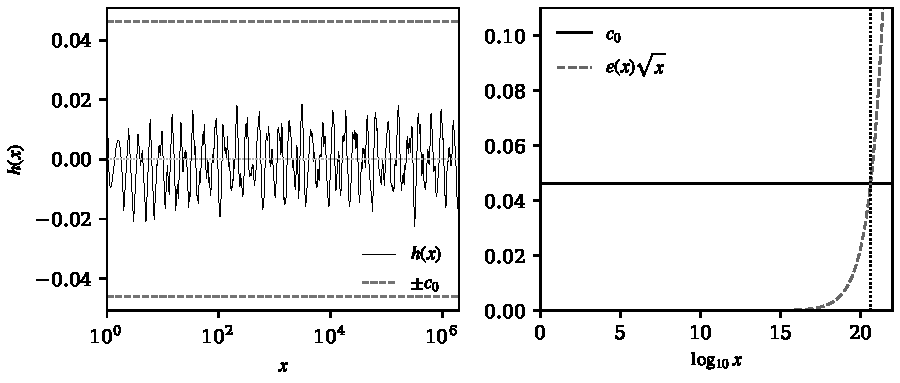
\includegraphics[width=\textwidth]{fig/zfb_bound.pdf}
\caption{Left: $(\mathcal G(x)-\log2\pi+\mathrm{tr}(x))/\sqrt x$ for $1.5\le x\le2\cdot10^6$, computed from the prime powers, between the lines $\pm F_0$ (at $x=1$ the value is $F_0$ exactly); its range is $[-0.0227,0.0187]$. Right: the two majorants of Theorem~\ref{mq:thm:uncond}, $F_0$ and $\varepsilon(x)\sqrt x$, they cross near $x=4.3\cdot10^{20}$.}\label{mq:fig:zfb}
\end{figure}

\begin{remark}[The lower limit under RH]\label{mq:rem:liminf3}
Under RH, $\liminf_{x\to\infty}\mathcal G(x)/\sqrt x\le f(\log3)<-0.0209$, and in fact $<-0.02268$ (below), where $f$ is the almost periodic function of Theorem~\ref{qt:thm:sharp}(2), $f(Y)=e^{-Y/2}(\mathcal G(e^Y)-\log2\pi+\mathrm{tr}(e^Y))$. This sharpens the bound $-0.0049990$ of Theorem~\ref{qt:thm:sharp}(2). Indeed $\sum_{n\le3}\Lambda(n)(3/n-1)=\tfrac12\log2$, so $\mathcal G(3)=\tfrac12\log2-3\log3+3(1+\gamma_E)=1.78238$, and $\mathcal G(3)-\log2\pi=-0.05549$. Further $\mathrm{tr}(3)\le\frac1{54}+\frac1{20}\sum_{k\ge2}9^{-k}=\frac1{54}+\frac1{1440}<0.019213$. Hence $f(\log3)<(-0.05549+0.019213)/\sqrt3<-0.0209$. For an almost periodic function the values near $f(\log3)$ recur on a relatively dense set, so $\liminf f\le f(\log3)$, and $\mathcal G(x)/\sqrt x-f(\log x)\to0$. The same argument at any other point gives a bound. At $x=319439$, the least value of $f(\log x)$ found on $1.5\le x\le2\cdot10^6$ (Figure~\ref{mq:fig:zfb}), the exact prime sum evaluated in interval arithmetic at $200$ bits gives $f(\log319439)\in-0.02268124049589\pm10^{-14}$, so under RH $\liminf_{x\to\infty}\mathcal G(x)/\sqrt x<-0.02268$. The enclosure is rigorous; that $319439$ is the least point of that range rests on a floating point scan, which the bound does not need.
\end{remark}

\subsection{Gaussian probes on one window}

The window criterion of Corollary~\ref{mq:hyp:window} uses infinitely many windows and is not effective. On one window a one sided bound still gives an explicit inequality. Write $g(u)=\mathcal G(e^u)$ and $\tilde g(u)=\sum_\rho a_\rho e^{\rho u}$ for real $u$, so that $\tilde g=g-\log2\pi+\mathrm{tr}(e^u)<g$ for $u\ge0$, and $|\tilde g(u)|\le C_0e^{\max(u,0)}$ for all $u$.

\begin{theorem}[Gaussian probes on one window]\label{mq:thm:gauss}
Let $\frac12\le\theta<1$, $Y\ge e^{12}$, $U=\log Y$, and suppose $\mathcal G(x)\le x^\theta$ for all $x\in[Y,Y^{3/2}]$. Put $u_0=\frac54U$ and $\tau^2=U/64$. Then for every $s=\sigma+it$ with $\frac12\le\sigma\le1$,
\[
\Bigl|\sum_\rho a_\rho e^{(\rho-s)u_0+(\rho-s)^2\tau^2/2}\Bigr|\le2.01\,W(\sigma),\qquad W(\sigma)=\exp\bigl(-(\sigma-\theta)u_0+\tfrac12(\sigma-\theta)^2\tau^2\bigr).
\]
\end{theorem}

\begin{proof}
Let $\varphi$ be the density of the normal law with mean $u_0$ and variance $\tau^2$, and $Z(s)=\int_{-\infty}^\infty\tilde g(u)e^{-su}\varphi(u)\,du$. Term by term, $Z(s)$ is the sum on the left. Since $|\tilde g|=2\max(\tilde g,0)-\tilde g$ and $Z(\sigma)$ is real,
\[
|Z(s)|\le2\int\max(\tilde g,0)\,e^{-\sigma u}\varphi\,du-Z(\sigma).
\]
\emph{The window.} For $U\le u\le\frac32U$, $\tilde g(u)<g(u)\le e^{\theta u}$, and $\int e^{(\theta-\sigma)u}\varphi\,du=W(\sigma)$. Note $W(\sigma)\ge e^{-u_0/2}=e^{-0.625U}$.

\emph{Outside.} With $c=1-\sigma\in[0,\frac12]$, the Gaussian tail bound gives
\[
\int_{u>3U/2}e^{cu}\varphi\,du\le\exp\Bigl(\tfrac32cU-\frac{U^2}{32\tau^2}\Bigr)\le e^{-1.25U},
\]
and the parts $0\le u<U$ and $u<0$ are at most $e^{-1.5U}$ and $e^{-49U}$. So the part outside the window is at most $3C_0e^{-1.25U}$.

\emph{The plain probe.} Write $d=\beta-\sigma\in(-1,\frac12]$. The term of $\rho$ in $Z(\sigma)$ has modulus at most $|a_\rho|\exp((\frac54d+\frac{d^2}{128})U-\frac{\gamma^2}{128}U)$. The function $\frac54d+d^2/128$ increases on $[-1,\frac12]$, so it is at most $0.625+0.25/128$ there, and every zero has $\gamma^2\ge14.13^2>199.65$. Hence
\[
|Z(\sigma)|\le C_0\exp\bigl([0.625+(0.25-199.65)/128]U\bigr)<C_0e^{-0.932U}.
\]
Together, $|Z(s)|\le W(\sigma)\,(2+7C_0e^{-0.307U})\le2.01\,W(\sigma)$ for $U\ge12$.
\end{proof}

\begin{corollary}[Dominant zeros]\label{mq:cor:dominant}
Under the hypotheses of Theorem~\ref{mq:thm:gauss}, let $\rho_0=\beta_0+i\gamma_0$ be a zero with $\beta_0>\theta$, and call it dominant at scale $Y$ if
\[
\sum_{\rho\ne\rho_0}|a_\rho|\exp\Bigl(\tfrac54(\beta-\beta_0)U+\frac{(\beta-\beta_0)^2-(\gamma-\gamma_0)^2}{128}\,U\Bigr)\le\tfrac12|a_{\rho_0}| ,
\]
the sum running over the zeros other than one chosen copy of $\rho_0$. Then
\[
\beta_0-\theta\le\frac{\log\bigl(4.02\,|\rho_0(1-\rho_0)|\bigr)}{1.246\,\log Y}.
\]
\end{corollary}

\begin{proof}
Take $s=\rho_0$ in the theorem. The term of $\rho_0$ is $a_{\rho_0}$ and the others sum to at most half of it in modulus, so $\frac12|a_{\rho_0}|\le2.01\exp(-(\beta_0-\theta)(\frac54-\frac1{256})U)$, because $(\beta_0-\theta)^2/128\le(\beta_0-\theta)/256$.
\end{proof}

So one window at scale $Y$ excludes dominant zeros in the region $\beta>\theta+{}$\allowbreak$0.81\log(4.02\gamma^2)/\log Y$.

\begin{theorem}[No lonely zeros]\label{mq:thm:lonely}
Under the hypotheses of Theorem~\ref{mq:thm:gauss}, let $\rho_0=\beta_0+i\gamma_0$ be a zero with
\[
\beta_0-\theta>\frac{\log\bigl(4.02\,|\rho_0(1-\rho_0)|\bigr)}{1.246\,\log Y},
\]
and let $n$ be the number of zeros $\rho$ with $|\gamma-\gamma_0|<13$. Then there is a zero other than one chosen copy of $\rho_0$ with
\[
|\gamma-\gamma_0|<13\qquad\text{and}\qquad\beta>\beta_0-\frac{\log(4n)}{1.24\,\log Y}.
\]
\end{theorem}

\begin{proof}
By conjugation take $\gamma_0>0$; then $\gamma_0>T_0$, because $\beta_0>\frac12$. Suppose the conclusion fails. We show that $\rho_0$ is dominant, which contradicts Corollary~\ref{mq:cor:dominant}. Write $\Delta\beta=\beta-\beta_0\in[-1,\frac12]$ and $\Delta\gamma=\gamma-\gamma_0$; the exponent in the definition of dominance is $E=U(\frac54\Delta\beta+\frac1{128}(\Delta\beta^2-\Delta\gamma^2))$.

\emph{Zeros with $|\Delta\gamma|\ge13$.} Here $E\le U(0.625+0.008-169/128)\le-0.687U$, so these zeros contribute at most $C_0e^{-0.687U}$. The assumption on $\beta_0$ and $\beta_0-\theta\le\frac12$ give $|\rho_0(1-\rho_0)|<e^{0.623U}/4.02$, hence $C_0e^{-0.687U}\le0.0115\,e^{-0.064U}|a_{\rho_0}|\le\frac18|a_{\rho_0}|$.

\emph{Zeros with $|\Delta\gamma|<13$.} By assumption each has $\Delta\beta\le-\lambda$ with $\lambda=\log(4n)/(1.24U)$. For $-1\le\Delta\beta\le0$, $\frac54\Delta\beta+\frac1{128}\Delta\beta^2\le-1.242|\Delta\beta|$, so $E\le-1.242\lambda U$ and $e^E\le1/(4n)$. Also $|a_\rho|\le(\gamma_0-13)^{-2}$. There are at most $n$ such zeros, so they contribute at most $\frac14(\gamma_0-13)^{-2}\le0.26\,|a_{\rho_0}|$, because $|a_{\rho_0}|^{-1}\le\gamma_0^2+1$ and $\gamma_0>T_0$.

The total is below $\frac12|a_{\rho_0}|$.
\end{proof}

\subsection{The effective criterion on one window}

\begin{lemma}[Gamma probes on one window]\label{mq:lem:gamma}
Let $\frac12\le\theta<1$, $U=\log Y\ge12$, and suppose $\mathcal G(x)\le x^\theta$ on $[Y,Y^{3/2}]$. Let $z=41+it$ with $t$ real, and let $k$ be an integer with $47.6\,U\le k\le50.8\,U$. Then
\[
\Bigl|\sum_\rho\frac{a_\rho}{(z-\rho)^k}\Bigr|\le\frac{2.07}{(41-\theta)^k}.
\]
\end{lemma}

\begin{proof}
For $\Re s>1$, $\int_0^\infty\tilde g(u)e^{-su}u^{k-1}\,du/(k-1)!=\sum_\rho a_\rho(s-\rho)^{-k}$, term by term. As in Theorem~\ref{mq:thm:gauss}, the modulus of the left side at $z$ is at most twice the integral of $\max(\tilde g,0)e^{-41u}u^{k-1}/(k-1)!$ less the value at $s=41$. On the window $\tilde g\le e^{\theta u}$, which gives at most $(41-\theta)^{-k}$. Outside, $|\tilde g|\le C_0e^u$, which gives $C_0\cdot40^{-k}$ times the probability that a Gamma variable of shape $k$ and rate $40$ falls outside $[U,\frac32U]$. Its mean $k/40$ lies in $[1.19U,1.27U]$, so by Chernoff's bound that probability is at most $2e^{-0.01428k}$. Since $(40.5/40)^k\le e^{0.01243k}$, the part outside is at most $2C_0e^{-0.00185k}(41-\theta)^{-k}$. At $s=41$ every $|41-\rho|\ge(40^2+\gamma_1^2)^{1/2}=42.42$, so that value is at most $C_0e^{-0.046k}(41-\theta)^{-k}$. With $k\ge47.6U$ and $U\ge12$ the total is at most $(2+4C_0e^{-0.088U}+C_0e^{-2U})(41-\theta)^{-k}\le2.07\,(41-\theta)^{-k}$.
\end{proof}

\emph{Tur\'an's second main theorem} (cited from S\'os and Tur\'an \cite{SosTuran55} and Tur\'an \cite{Turan84}). Let $b_1,\dots,b_n$ and $\zeta_1,\dots,\zeta_n$ be complex numbers with $1=|\zeta_1|\ge|\zeta_2|\ge\cdots\ge|\zeta_n|$, and let $m\ge0$ be an integer. Then there is an integer $\nu$ with $m+1\le\nu\le m+n$ and
\[
\Bigl|\sum_{i=1}^nb_i\zeta_i^\nu\Bigr|\ge2\Bigl(\frac n{8e(m+n)}\Bigr)^n\min_{1\le j\le n}|b_1+\cdots+b_j| .
\]

\begin{theorem}[Effective criterion on one window]\label{mq:thm:effective}
Let $\frac12\le\theta<1$, $U=\log Y\ge12$, and suppose $\mathcal G(x)\le x^\theta$ for all $x\in[Y,Y^{3/2}]$. Let $\rho_0=\beta_0+i\gamma_0$ be a zero with $\beta_0>\theta$, and let $N\ge1$ be an upper bound for the number of zeros $\rho$ with $\beta>\theta$ and $|\gamma-\gamma_0|<6.35$, with $N\le U/10$. Then
\[
\beta_0-\theta\le\frac{\log(1.07\,\gamma_0^2)+5.88\,N}{1.175\,\log Y}\qquad(\gamma_0>0).
\]
\end{theorem}

\begin{proof}
By conjugation $\gamma_0>0$, and $\gamma_0>T_0$. Let $z=41+i\gamma_0$ and let $\mathcal N_z$ be the set of zeros with $|z-\rho|<41-\theta$, counted with multiplicity, $n=|\mathcal N_z|$. For $\rho$ in $\mathcal N_z$, $41-\beta<41-\theta$, so $\beta>\theta$, and $(\gamma-\gamma_0)^2<(\beta-\theta)(82-\beta-\theta)\le40.25$, so $|\gamma-\gamma_0|<6.35$. Hence $\rho_0\in\mathcal N_z$ and $1\le n\le N$.

\emph{The upper bound.} The zeros outside $\mathcal N_z$ contribute at most $C_0(41-\theta)^{-k}$ to the sum of Lemma~\ref{mq:lem:gamma}. So for every integer $k$ in $[47.6U,50.8U]$
\[
\Bigl|\sum_{\rho\in\mathcal N_z}\frac{a_\rho}{(z-\rho)^k}\Bigr|\le\frac{2.12}{(41-\theta)^k}.
\]

\emph{The progression.} Let $p=\lfloor3.2U/N\rfloor$; since $N\le U/10$, $p\ge3.1U/N\ge31$. Let $m+1=\lceil47.6U/p\rceil$. For $m+1\le\nu\le m+n$ the integer $k=p\nu$ satisfies $47.6U\le k\le47.6U+pn\le50.8U$. So the lemma applies to all these $k$, and $m+n\le50.8U/p\le(50.8/3.1)N$.

\emph{The power sum.} Order $\mathcal N_z$ by increasing distance from $z$, let $d_1$ be the least distance and $\rho_1$ a zero at that distance, and put $\zeta_i=(d_1/(z-\rho_i))^p$ and $b_i=a_{\rho_i}$. Then $\sum_{\rho\in\mathcal N_z}a_\rho(z-\rho)^{-p\nu}=d_1^{-p\nu}\sum_ib_i\zeta_i^\nu$. Every zero of $\mathcal N_z$ has $\gamma>T_0$, so the argument of $a_\rho$ is below $10^{-12}$ in modulus, and every partial sum satisfies $|b_1+\cdots+b_j|\ge0.999\,|a_{\rho_1}|$. Put $C=8e\,(50.8/3.1)<356.36$, so that $\log C<5.876$. Tur\'an's theorem gives $\nu$ in the range, and so $k=p\nu$, with
\[
\Bigl|\sum_{\rho\in\mathcal N_z}\frac{a_\rho}{(z-\rho)^k}\Bigr|\ge\frac{1.99\,|a_{\rho_1}|}{d_1^{\,k}}\Bigl(\frac n{CN}\Bigr)^n\ge\frac{1.99\,|a_{\rho_1}|}{d_1^{\,k}}\,e^{-5.876N},
\]
because $n\log(CN/n)$ increases with $n$ up to $n=N$.

\emph{Conclusion.} Comparing, $((41-\theta)/d_1)^k\le1.066\,|a_{\rho_1}|^{-1}e^{5.876N}$. Here $d_1\le41-\beta_0$, so the left side is at least $\exp(k(\beta_0-\theta)/40.5)\ge\exp(1.175(\beta_0-\theta)U)$. And $|a_{\rho_1}|^{-1}=|\rho_1(1-\rho_1)|\le(\gamma_0+7)^2+1\le1.001\gamma_0^2$, and $1.066\cdot1.001<1.07$.
\end{proof}

\begin{lemma}[A local zero count]\label{mq:lem:count}
For $t>T_0$ the number of zeros $\rho$, counted with multiplicity, with $|\gamma-t|<6.35$ is at most $2.25\log t+6$.
\end{lemma}

\begin{proof}
Let $h=6.35$, $L=\log t$, $P(\tau)=\tau\log(\tau/2\pi e)/(2\pi)$, and let $N_+(\tau)$ count the zeros with $0<\gamma\le\tau$. By the Riemann von Mangoldt formula $N_+(\tau)=P(\tau)+\frac78+S(\tau)+O^*(1/(5\tau))$, and by the second branch of Corollary~1.4 of Hasanalizade, Shen and Wong \cite{HSW22}, $|S(\tau)|\le0.1095\log\tau+0.2042\log\log\tau+3.0305$ at the heights used here. The interval $(t-h,t+h)$ lies in the positive ordinates, and the number of zeros in it is at most $N_+(t+h)-N_+(t-h)$. The main increment is $P(t+h)-P(t-h)\le(h/\pi)\log((t+h)/2\pi)<2.0213L-3.715$. The two values of $S$ contribute at most $2(0.1095L+0.2042\log L+3.0305)=0.219L+0.4084\log L+6.061$, the changes from replacing $\log(t\pm h)$ by $\log t$ being below $10^{-10}$, and the remainders $O^*(1/(5\tau))$ contribute below $10^{-12}$. The sum is at most $2.2403L+0.4084\log L+2.35\le2.25L+6$, because $0.0097L+3.65-0.4084\log L\ge2.4$ for $L\ge28.7$.
\end{proof}

\begin{corollary}[A zero free region from one window]\label{mq:cor:region}
Let $\frac12\le\theta<1$, $U=\log Y\ge12$, and suppose $\mathcal G(x)\le x^\theta$ on the single window $[Y,Y^{3/2}]$. Then $\zeta$ has no zero in the region
\[
\beta>\theta+\frac{13\log|\gamma|+30.2}{\log Y},\qquad \log|\gamma|\le\frac{\log Y}{25}.
\]
\end{corollary}

\begin{proof}
Let $\rho_0$ be a zero with $\beta_0>\theta$, so that $|\gamma_0|>T_0$; take $\gamma_0=t>0$ by conjugation. If $U<600$, then $\log t\le U/25<24<\log T_0$, so there is no such zero in the region. Let $U\ge600$ and $\log t\le U/25$. Lemma~\ref{mq:lem:count} allows $N=2.25\log t+6$, and $N\le0.09U+6\le U/10$. The numerator of Theorem~\ref{mq:thm:effective} is $\log(1.07)+2\log t+5.88N\le15.23\log t+35.4$, and $15.23/1.175<13$, $35.4/1.175<30.2$.
\end{proof}

So the excluded region has the shape $\beta>\theta+C\log\gamma/\log Y$ with $C=13$ and no isolation assumed; the Gaussian probes of Corollary~\ref{mq:cor:dominant} give the same shape with $C\approx1.62$ for dominant zeros. With $p(U,\delta)=\min\{\frac1{25},(\delta-30.2/U)/13\}$ the window excludes every zero to the right of $\theta+\delta$ up to the height $H=Y^{p}$, which is new only if $Up>\log T_0$. For $\log Y=10^5$ and $\delta=\frac14$ the computed value is $p>0.0192$.
The infinite criterion follows at once: if the bound holds on windows at arbitrarily large $Y$, the right side of Theorem~\ref{mq:thm:effective} tends to zero for each fixed zero, so there is no zero to the right of $\theta$.

\begin{remark}[Literature]\label{mq:rem:zfblit}
The method is Landau's argument made explicit by Tur\'an's power sums, as used by Tur\'an \cite{Turan50}, Pintz \cite{Pintz80}, Schlage-Puchta \cite{SchlagePuchta} and R\'ev\'esz \cite{Revesz23} for $\psi(x)-x$; see also Remark~\ref{mq:rem:windowlit}. We have not compared the constants with that literature, and we make no claim of novelty or priority.
\end{remark}

\section{The Brownian form of the slack}\label{mq:sec:brownian}

\subsection{The resolvent family}

For $a>\frac12$ and $u\in\mathbb R$ put
\begin{align*}
W_a(u)&=\sum_\rho\frac{e^{(\rho-1/2)u}}{a^2+\tau_\rho^2}=\sum_\rho\frac{\cos(\tau_\rho u)}{a^2+\tau_\rho^2},\\
c(a)&=W_a(0)=\frac1a\,\frac{\xi'}{\xi}\Big(\frac12+a\Big),\qquad\Phi_a(u)=W_a(0)-W_a(u),
\end{align*}
the zero part of the statistic $S_a$ of Proposition~\ref{qt:prop:laplace}, normalised so that $2aW_a=D_a+T_a$ in the notation there. The two forms of $W_a$ agree because the zero set is invariant under $\rho\mapsto1-\rho$, and the sums converge absolutely because $\Re(a^2+\tau_\rho^2)\ge a^2+\gamma^2-\frac14>0$. For $a=\frac12$ and $u\ge0$, $W_{1/2}(u)=e^{-u/2}(\mathcal G(e^u)-\log2\pi+\mathrm{tr}(e^u))$ is the function $f$ of Theorem~\ref{qt:thm:sharp}(2), $c(\frac12)=F_0$ and $\Phi_{1/2}$ is the slack $\Phi$ of Section~\ref{st:sec:riesz}. Unconditionally $\Phi_a(u)=\sum_\rho(1-\cos\tau_\rho u)/(a^2+\tau_\rho^2)$, and under RH every term is nonnegative.

\begin{proposition}[The criterion at every width]\label{mq:prop:crit}
Let $a>\frac12$, $a\notin\{\frac52,\frac92,\dots\}$. Then RH holds if and only if $\Phi_a(u)\ge0$ for all $u\ge0$.
\end{proposition}

\begin{proof}
Under RH $\tau_\rho$ is real and each term of $\Phi_a$ is nonnegative. Conversely $\Phi_a\ge0$ says $W_a(u)\le c(a)$, hence $D_a(u)=2aW_a(u)-T_a(u)\le2ac(a)+\sup_{u\ge0}|T_a|$, a bound for $D_a$ of the form $Ke^{0\cdot u}$, because $T_a$ is bounded on $[0,\infty)$ for $a>\frac12$, $a\notin\{\frac52,\frac92,\dots\}$. By Proposition~\ref{qt:prop:laplace} with $\theta=\frac12$ no zero has $\Re\rho>\frac12$.
\end{proof}

\subsection{The Brownian form}

Let $\tau_v$ be the first passage time of standard Brownian motion over a distance $|v|$, so that $\mathbb E\,e^{-\lambda\tau_v}=e^{-\sqrt{2\lambda}|v|}$, which at $\lambda=a^2/2$ is $e^{-a|v|}$.

\begin{theorem}[Brownian form]\label{mq:thm:brownian}
Let $a>\frac12$ and $u\ge0$. Unconditionally,
\[
W_a(u)=\frac{8\cosh(u/2)}{4a^2-1}-\frac1{2a}\sum_n\frac{\Lambda(n)}{\sqrt n}\Big(e^{-a|u-\log n|}+e^{-a(u+\log n)}\Big)+B_a(u),
\]
\[
B_a(u)=-\frac{e^{-au}\log\pi}{2a}+\frac1{2\pi}\int_{-\infty}^\infty\frac{\cos(ur)}{a^2+r^2}\,\Re\,\psi\Big(\frac14+\frac{ir}2\Big)dr,
\]
where $\psi$ is the digamma function. The sum converges absolutely, since its terms are $O(\Lambda(n)n^{-1/2-a})$.
\end{theorem}

\begin{proof}
Apply Weil's explicit formula \cite{Weil52} in the form $\sum_\rho h(\tau_\rho)=h(\frac i2)+h(-\frac i2)-g(0)\log\pi+\frac1{2\pi}\int h(r)\Re\psi(\frac14+\frac{ir}2)dr-2\sum_n\Lambda(n)n^{-1/2}g(\log n)$ to $g(v)=\frac12(e^{-a|u-v|}+e^{-a|u+v|})$, which is even, with $h(r)=\int g(v)e^{irv}dv=\frac{2a\cos(ur)}{a^2+r^2}$. The formula applies because $g(v)e^{(1/2+\delta)|v|}$ is integrable for $0<\delta<a-\frac12$ and $h$ is holomorphic in $|\Im r|<a$. Then $h(\pm\frac i2)=\frac{2a\cosh(u/2)}{a^2-1/4}$ and $g(0)=e^{-au}$. The zero sum is $2aW_a(u)$, and dividing by $2a$ gives the formula.
\end{proof}

Subtracting from the value at $u=0$ gives the prime form of the slack. Put, for $u>0$ and $y\ge0$,
\[
\kappa_a(u,y)=2e^{-ay}-e^{-a|u-y|}-e^{-a(u+y)},
\]
minus the second difference with step $u$ of the Brownian passage kernel $e^{-a|\cdot|}$ at $y$.

\begin{corollary}[Prime form of the slack]\label{mq:cor:primeslack}
For $a>\frac12$ and $u>0$,
\[
\Phi_a(u)=-\frac1{2a}\sum_n\frac{\Lambda(n)}{\sqrt n}\,\kappa_a(u,\log n)-\frac{16\sinh^2(u/4)}{4a^2-1}+B_a(0)-B_a(u).
\]
For fixed $u>0$, $\kappa_a(u,y)>0$ exactly when $y<y^*(u)=\frac1{2a}\log(2e^{au}-1)$, and $y^*(u)=\frac u2+\frac{\log2}{2a}+o(1)$ as $u\to\infty$. The point $y^*$ lies in $(0,u)$.
\end{corollary}

\begin{proof}
Subtract the formula of Theorem~\ref{mq:thm:brownian} at $u$ from its value at $0$, where the prime terms are $2e^{-a\log n}$, and use $1-\cosh(u/2)=-2\sinh^2(u/4)$. For $y\ge u$, $\kappa_a=-e^{-ay}(e^{au/2}-e^{-au/2})^2<0$. For $0\le y<u$, $\kappa_a=e^{-ay}(2-e^{-au})-e^{-au}e^{ay}$ is strictly decreasing in $y$, positive at $y=0$ and negative at $y=u$, and vanishes where $e^{2ay}=2e^{au}-1$, which is below $e^{2au}$ because $(e^{au}-1)^2>0$.
\end{proof}

\begin{theorem}[Prime form of RH]\label{mq:thm:primeform}
Let $a>\frac12$, $a\notin\{\frac52,\frac92,\dots\}$. RH holds if and only if for every $u>0$
\[
\sum_n\frac{\Lambda(n)}{\sqrt n}\,\kappa_a(u,\log n)\ \le\ 2a\big[B_a(0)-B_a(u)\big]-\frac{32a\,\sinh^2(u/4)}{4a^2-1}.
\]
Under an analogue of Corollary~\ref{mq:hyp:window} for the statistic $S_a$ (not proved here, and used only as a hypothesis), it suffices that the inequality hold up to an additive error $e^{\epsilon u}$, for every $\epsilon>0$, on windows $u\in[U,\frac32U]$ with $U$ arbitrarily large.
\end{theorem}

\begin{proof}
By Corollary~\ref{mq:cor:primeslack} the displayed inequality is $\Phi_a(u)\ge0$, and Proposition~\ref{mq:prop:crit} gives the equivalence. For the second sentence, $\Phi_a(u)\ge-e^{\epsilon u}$ on windows is the window bound for $D_a$ at exponent $\frac12+\epsilon$, and the assumed analogue of (W) for $S_a$ then gives no zero with $\Re\rho>\frac12+\epsilon$.
\end{proof}

\subsection{The size biased reading of the tilted zero law}

Assume RH, so that $\tau_\rho=\gamma$ is real, and let the ordinates $\gamma>0$ be repeated with multiplicity. The sum of the weights $\nu_a=\sum_\rho(a^2+\gamma_\rho^2)^{-1}\delta_{\gamma_\rho}$ over all zeros is $c(a)$, and $W_a(u)=\int\cos(ur)\,\nu_a(dr)$, $\Phi_a(u)=\int(1-\cos ur)\,\nu_a(dr)$ with a finite positive measure $\nu_a$. Let $E_\gamma$ be independent exponential variables of rate $(a^2+\gamma^2)/2$, one for each ordinate $\gamma>0$ with multiplicity, and $\mathcal T_a=\sum_{\gamma>0}E_\gamma$. By Hadamard's product $\xi(\frac12+s)/\xi(\frac12)=\prod_{\gamma>0}(1+s^2/\gamma^2)$ (the function is even, entire of order one) the variable $\mathcal T_a$ has mean $\sum_{\gamma>0}2/(a^2+\gamma^2)=c(a)$, and $a=\frac12$ is the case of $F_0$.

\begin{lemma}[Size biasing a sum of exponentials]\label{mq:lem:sizebias}
Let $\mathcal T=\sum_kE_k$ with independent $E_k$ of rates $r_k>0$ and $\sum_k1/r_k<\infty$. The size biased law $\hat{\mathcal T}$, with density $t\,f_{\mathcal T}(t)/\mathbb E\mathcal T$, is that of $\mathcal T+E'_K$, where $\mathbb P(K=k)=r_k^{-1}/\sum_jr_j^{-1}$ and, given $K$, $E'_K$ is exponential of rate $r_K$, independent of $\mathcal T$.
\end{lemma}

\begin{proof}
For $\lambda\ge0$, $\mathbb E[\mathcal Te^{-\lambda\mathcal T}]/\mathbb E\mathcal T=\mathbb Ee^{-\lambda\mathcal T}\,\sum_k(r_k+\lambda)^{-1}\big/\sum_jr_j^{-1}=\mathbb Ee^{-\lambda\mathcal T}\,\mathbb E\big[r_K/(r_K+\lambda)\big]$, and $r_K/(r_K+\lambda)$ is the transform of $E'_K$.
\end{proof}

\begin{proposition}[Size biased reading]\label{mq:prop:sizebias}
Assume RH. Let $K_a$ be the ordinate selected by size biasing $\mathcal T_a$, so that $\mathbb P(K_a=\gamma)\propto m_\gamma/(a^2+\gamma^2)$ for $\gamma>0$ with multiplicity $m_\gamma$. Then $W_a(u)=c(a)\,\mathbb E\cos(\gamma_{K_a}u)$ and $\Phi_a(u)=c(a)\,\mathbb E\big[2\sin^2(\gamma_{K_a}u/2)\big]$.
\end{proposition}

\begin{proof}
By Lemma~\ref{mq:lem:sizebias} with $r_\gamma=(a^2+\gamma^2)/2$ the probability of the summand $E_\gamma$ is proportional to $2/(a^2+\gamma^2)$, with normaliser $c(a)$, and $W_a(u)=\sum_{\gamma>0}2\cos(\gamma u)/(a^2+\gamma^2)$ under RH.
\end{proof}

We use only the elementary exponential sum law of $\mathcal T_a$, and make no claim that it is the hitting time of a one dimensional diffusion; with multiplicities and a reflecting end that identification fails.

\section{The frame model}\label{mq:sec:frame}

This section computes, for arbitrary weights, what the reported shape of the data of (M) implies, in a model: the frame below is inferred from the numerology of (M), namely $2n$ cells, an average over a group of order $n$, a Behrend set of density $\delta=|T_2|/n$ and a family of $4n$ characters, and it has not been checked against the formal development of the claimed proof. Every theorem in this section is correct within the model and for the standard frame defined below only (a more general notion of frame admits counterexamples, see the remark after the definition), and none of them is a statement about the claimed proof itself.

\begin{lemma}[The excluded primes carry no weight]\label{mq:lem:congruence}
Let $q\equiv3\pmod8$ and $d\equiv7\pmod8$ be primes with $q\mid d+1$. Then $\chi_d(2)=\chi_d(q)=1$ and $\chi_q(2)=-1$. Consequently $1-\chi_d(r)=0$ for every power $r$ of $2$ or of $q$, and so does the Chebyshev weight $(1+\chi_q(r))(1-\chi_d(r))$.
\end{lemma}

\begin{proof}
$\chi_d$ is the Kronecker symbol of the discriminant $-d\equiv1\pmod8$, so $\chi_d(2)=1$. Since $d\equiv-1\pmod q$, $-d\equiv1\pmod q$ and $\chi_d(q)=\big(\frac1q\big)=1$. The discriminant $-q\equiv5\pmod8$ gives $\chi_q(2)=-1$.
\end{proof}

\begin{definition}[Standard frame]\label{mq:def:frame}
Let $N=4nq$ and let $C_n$ be the cyclic quotient of $(\mathbb Z/4n\mathbb Z)^\times$ by $\{\pm1\}$. The standard frame is the group $\mathsf G=C_n\times\{\pm1\}$ with the map $r\mapsto[r]=(r\bmod4n,\chi_q(r))\in\mathsf G$ on the prime powers $r$ prime to $N$, where $r\bmod4n$ is read in $C_n$. Its elements are the cells, there are $2n$ of them, and the map is induced by a surjective homomorphism $(\mathbb Z/N\mathbb Z)^\times\to\mathsf G$ (surjective by the Chinese remainder theorem). The characters of $\mathsf G$ are $\xi\chi_q^i$ with $\xi$ even modulo $4n$ and $i\in\{0,1\}$, each composed with this map is a Dirichlet character modulo $N$, and $H=\ker\chi_q\cong C_n$ has index $2$, so that the characters trivial on $H$ are exactly $1$ and $\chi_q$.
\end{definition}

The standard frame has the property that $1-\chi_d(r)=0$ for every prime power $r$ not prime to $N$, by Lemma~\ref{mq:lem:congruence}, since the primes dividing $N=4nq$ are $2$ and $q$; this is what the theorems below use. A more general notion, a finite abelian group $\mathsf G$ with a map from the prime powers such that every character composes to a Dirichlet character, is not adequate: for $N=1$, $\mathsf G=\{\pm1\}$ and every prime power mapped to $+1$, both characters pull back to the trivial character and the identity of Theorem~\ref{mq:thm:celldecomp} fails for unequal weights (the two sides differ by $a(\langle\log w\rangle-\log w_+)$). In the frame model a weight system is a map $w:\mathsf G\to(0,\infty)$ with $X_g=a/w_g\ge1$ (the data of (M) have this property), and $P$, $M$ are as in Section~\ref{mq:sec:setting} with $w_{\mathrm{cell}(r)}$ replaced by $w_{[r]}$.

\begin{theorem}[Exact cell decomposition]\label{mq:thm:celldecomp}
For arbitrary weights on the standard frame,
\[
P-M=\frac1{|\mathsf G|}\sum_{g\in\mathsf G}w_g\sum_{\xi\in\widehat{\mathsf G}}\overline\xi(g)\Big[\mathcal G_\xi(X_g)-\mathcal G_{\xi\chi_d}(X_g)\Big].
\]
Here $\xi$ may be read as induced modulo $N$ or as its primitive associate, and for $\xi$ trivial as the zeta statistic rather than the principal character modulo $N$: only the difference $\mathcal G_\xi-\mathcal G_{\xi\chi_d}$ occurs, and it is the same in all readings, because $1-\chi_d$ vanishes on the powers of $2$ and $q$ (the individual Euler factors at $2$ and $q$ do differ).
\end{theorem}

\begin{proof}
By Lemma~\ref{mq:lem:congruence} the weight $1-\chi_d(r)$ vanishes for $r$ not prime to $N$, so $P$ may be taken over all prime powers $r$, and $(a/r-w)_+=w(X/r-1)_+$ with $X=a/w$. Orthogonality, $\mathbf 1\{[r]=g\}=\frac1{|\mathsf G|}\sum_\xi\overline\xi(g)\xi(r)$, gives
\[
P=\frac1{|\mathsf G|}\sum_gw_g\sum_\xi\overline\xi(g)\sum_r\Lambda(r)\,\xi(r)\big(1-\chi_d(r)\big)\Big(\frac{X_g}r-1\Big)_+ .
\]
For nontrivial $\xi$ (the terms with $r$ not prime to $N$ have weight zero) the inner sum is $\mathcal G_\xi(X_g)-\mathcal G_{\xi\chi_d}(X_g)-X_g\big[\frac{L'}{L}(1,\xi)-\frac{L'}{L}(1,\xi\chi_d)\big]$. Here $\xi\chi_d$ is not principal, since $d$ is a prime distinct from $2$ and $q$ and so does not divide $4nq$. Since $w_gX_g=a$ for all $g$, the bracket enters $P$ multiplied by $\frac a{|\mathsf G|}\sum_g\overline\xi(g)=0$. For trivial $\xi$ (the principal character modulo $N$ gives the same inner sum, the extra terms having weight zero) the inner sum is $S(X_g)-S_{\chi_d}(X_g)$ with $S_\psi(X)=\sum_r\Lambda(r)\psi(r)(X/r-1)_+$, and from \eqref{mq:eq:Gpsi},
\[
w_g\big[S(X_g)-S_{\chi_d}(X_g)\big]=w_g\big[\mathcal G(X_g)-\mathcal G_{\chi_d}(X_g)\big]+a\Big[\log\frac a{w_g}-1-\gamma_E+\frac{L'}L(1,\chi_d)\Big].
\]
Averaging the last bracket over $g\in\mathsf G$ gives exactly $M$.
\end{proof}

For $u\in\mathsf G$ let $P_u$ be the prime sum with the translated weights $w^u_g=w_{gu^{-1}}$; the average $\langle\log w\rangle$ and so $M$ do not change.

\begin{theorem}[Averaged identity]\label{mq:thm:averaged}
Let $\mathsf G$ be the standard frame and $H=\ker\chi_q$, so that the characters trivial on $H$ are exactly $1$ and $\chi_q$. Let $D\subseteq H$ and $\delta=2|D|/|\mathsf G|$. Suppose (i) $b\le w_g\le b(1+\eta)$ for $g\in D$, (ii) $a/w_g\ge y_0$ for $g\notin D$, and (iii) $|\mathcal G_\psi(y)|\le y\vartheta$ for all $y\ge y_0$ and $\psi\in\{1,\chi_q,\chi_d,\chi_q\chi_d\}$. Then with $x=a/b$,
\[
\frac1{|H|}\sum_{u\in H}\big(P_u-M\big)=\frac{b\delta}2\Big[R_{q,d}(x)+\mathcal E\Big],\qquad|\mathcal E|\le\frac{8x\vartheta}\delta+12\,x\,\eta .
\]
For data of this shape, with all $(t,j)$ sharing the same $b$, $\delta$ and scale $x=a/b$, and (i) to (iii) holding uniformly in $(t,j)$, summing over $t\in T$ and $j\le m$ gives $B\,(R_{q,d}(x)+\mathcal E)$ with $B=|T|\,m\,b\,\delta/2$ and the same bound for $|\mathcal E|$.
\end{theorem}

\begin{proof}
Apply Theorem~\ref{mq:thm:celldecomp} to the weights $w^u$ and substitute $g=g'u$:
\[
P_u-M=\frac1{|\mathsf G|}\sum_{g'}w_{g'}\sum_\xi\overline\xi(g')\,\overline\xi(u)\Big[\mathcal G_\xi(X_{g'})-\mathcal G_{\xi\chi_d}(X_{g'})\Big].
\]
Averaging over $u\in H$ replaces $\overline\xi(u)$ by $1$ if $\xi$ is trivial on $H$ and by $0$ otherwise, so only $\xi\in\{1,\chi_q\}$ survive:
\[
\frac1{|H|}\sum_{u\in H}(P_u-M)=\frac1{|\mathsf G|}\sum_gw_g\Big[F_1(X_g)+\chi_q(g)F_{\chi_q}(X_g)\Big],\qquad F_\xi=\mathcal G_\xi-\mathcal G_{\xi\chi_d}.
\]
Cells outside $D$: each term is at most $w_g\cdot4X_g\vartheta=4a\vartheta$ in modulus by (ii) and (iii), so their total is at most $4a\vartheta=\frac{b\delta}2\cdot\frac{8x\vartheta}\delta$. Cells in $D$ with $w_g=b$ exactly: $\chi_q(g)=1$ and $X_g=x$, so each contributes $\frac b{|\mathsf G|}\big[\mathcal G(x)-\mathcal G_{\chi_d}(x)+\mathcal G_{\chi_q}(x)-\mathcal G_{\chi_q\chi_d}(x)\big]=\frac b{|\mathsf G|}R_{q,d}(x)$, and there are $|D|=\delta|\mathsf G|/2$ of them. Moving the weights to $b$: for nonprincipal $\psi$, $w\,\mathcal G_\psi(a/w)=\sum_r\Lambda(r)\psi(r)(a/r-w)_++a\frac{L'}L(1,\psi)$ has derivative $-\sum_{r\le a/w}\Lambda(r)\psi(r)$ in $w$ (one sided at the breakpoints $w=a/r$, where the function is absolutely continuous, so the Lipschitz estimate below is valid), and for the trivial character the derivative is $x'-\psi(x')$ with $x'=a/w$ and $\psi$ Chebyshev's function. By the bound $\psi(y)\le1.04y$ of Rosser and Schoenfeld \cite{RS62} both are at most $3x$ in modulus for $w\ge b$. Each distinguished cell carries four such statistics, so replacing $w_g$ by $b$ changes the sum by at most $\frac{|D|}{|\mathsf G|}\cdot4\cdot3x\cdot b\eta=\frac{b\delta}2\cdot12x\eta$.
\end{proof}

With the reported parameters the error is negligible: $\eta=O(1/(nx^2))$ gives $12x\eta=O(1/(nx))$, and $\vartheta=\exp(-\kappa x^{\epsilon/8})$ with $\delta\ge x^{-\epsilon}$ gives $8x\vartheta/\delta=o(1)$. The shape of the data assumed (the dependence on $u$ a translation of the distinguished cells on a frame, the two level form (i), (ii), and a common scale $x=a/b$ for all $(t,j)$) has not been checked against the construction in the draft; Theorem~\ref{mq:thm:link4} below drops the requirement that the weights themselves are translates and lets $a_t/b$ differ from $x$ by at most $1$.

Theorem~\ref{mq:thm:averaged} assumes that the weights of the tables are translates of one system. The next theorem is an algebraic form, with explicit constants and proved here, of the passage from (M) to the bound for $\mathcal G$ reported in \cite{Rub26}. It needs less: the weights may be arbitrary for each $(u,t,j)$, only the set of distinguished cells moves by translation with $u$, there are several labels $t$ with different parameters $a_t$, and $a_t/b$ has to lie within $1$ of $x$. The price is that all $4n$ characters of the frame and their $\chi_d$ twists enter (Estimate C covers them, Theorem~\ref{mq:thm:estC}), which costs a factor $n$ in the $\vartheta$ term, and a constant $17\log(x+1)+7$ from moving $a_t/b$ to $x$. Write $\lambda_\psi=\frac{L'}{L}(1,\psi)$ and $F_\xi=\mathcal G_\xi-\mathcal G_{\xi\chi_d}$.

\begin{theorem}[From (M) to the residue sum, general weights]\label{mq:thm:link4}
Let $\mathsf G$ be the standard frame, $H=\ker\chi_q$ and $x\ge3$. Let $T$ be a finite set, $m\ge1$ an integer, $a_t>0$ for $t\in T$, $b>0$, $0<\delta\le1$, and for each $(t,j)$ a set $D_{t,j}\subseteq H$ with $|D_{t,j}|=\delta n$. For $u\in H$, $t\in T$ and $1\le j\le m$ let $w^{u,t,j}:\mathsf G\to(0,\infty)$ be arbitrary weights, and let $P_{u,t,j},M_{u,t,j}$ be the quantities of Theorem~\ref{mq:thm:celldecomp} for these weights and the parameter $a_t$. The cells of $uD_{t,j}$ are called distinguished at $(u,t,j)$. Put $B=|T|mb\delta/2$ and suppose, with numbers $\Delta\ge0$, $y_0\ge1$, $\vartheta\ge0$ and $E$:
\begin{enumerate}
\item[(a)] $|a_t/b-x|\le1$ for $t\in T$;
\item[(b)] $b\le w^{u,t,j}_g\le b(1+\Delta)$ at the distinguished cells and $a_t/w^{u,t,j}_g\ge y_0$ at all other cells;
\item[(c)] $|\mathcal G_\psi(y)|\le\vartheta y$ for $y\ge y_0$ and each of the $4n$ characters $\psi=\xi\chi_d^l$, with $\xi\in\widehat{\mathsf G}$ and $l\in\{0,1\}$;
\item[(d)] $|\lambda_\psi|\le4\log x$ for $\psi=\chi_q,\chi_d,\chi_q\chi_d$;
\item[(M$'$)] $\displaystyle\frac1n\sum_{u\in H}\sum_{t\in T}\sum_{j=1}^m\big(P_{u,t,j}-M_{u,t,j}\big)\le E$.
\end{enumerate}
Then
\[
R_{q,d}(x)\le\frac EB+\frac{8n(x+1)\vartheta}{\delta}+\frac{5.2\,(x+1)\Delta}{\delta}+17\log(x+1)+7 .
\]
\end{theorem}

\begin{proof}
Fix a table $(u,t,j)$, write $w=w^{u,t,j}$, $a=a_t$ and $\mu=1/(2n)$. By Theorem~\ref{mq:thm:celldecomp}, $P-M=\sum_{g\in\mathsf G}T_g$ with $T_g=\mu\,w_g\sum_\xi\overline\xi(g)F_\xi(a/w_g)$.

\emph{Other cells.} By (b) and (c), $|F_\xi(a/w_g)|\le2\vartheta a/w_g$, so $|T_g|\le2a\vartheta\le2b(x+1)\vartheta$ by (a). At most $2n$ cells are not distinguished, in each of the $n|T|m$ tables, so their part of the mean in (M$'$) is at most $|T|m\cdot4nb(x+1)\vartheta=B\cdot8n(x+1)\vartheta/\delta$ in modulus.

\emph{Distinguished cells, weights moved to $b$.} Write $c(r)=(1-\chi_d(r))\Lambda(r)$. The proof of Theorem~\ref{mq:thm:celldecomp} shows $T_g(w_g)=\sum_{[r]=g}c(r)(a/r-w_g)_+-\mu\,a\,(\log(a/w_g)+K_g)$ with $K_g$ independent of $a$ and $w_g$. For $b\le w_g\le b(1+\Delta)$ the first sum changes by at most $b\Delta\sum_{r\le a/b,\,[r]=g}c(r)$ when $w_g$ is replaced by $b$ (the terms with $r>a/b$ vanish at both weights), and the second by at most $\mu a\Delta$. Over the $\delta n$ distinguished cells of one table, with $c(r)\le2\Lambda(r)$, $a/b\le x+1$, $\delta\le1$ and $\psi(y)\le1.04y$ \cite{RS62}, the total change is at most $b\Delta\big(2\psi(x+1)+\frac\delta2(x+1)\big)\le2.6\,b\Delta(x+1)$. As before this gives a part of the mean of modulus at most $B\cdot5.2(x+1)\Delta/\delta$.

\emph{Translation.} With weight $b$ at the distinguished cells, $T_g=\mu b\sum_\xi\overline\xi(g)F_\xi(y)$ with $y=a_t/b$, and the sum over $g\in uD_{t,j}$ averaged over $u\in H$ keeps only the $\xi$ trivial on $H$, that is $\xi\in\{1,\chi_q\}$, for which $\xi(g)=1$ on $H$:
\[
\frac1n\sum_{u\in H}\sum_{g\in uD_{t,j}}\mu b\sum_\xi\overline\xi(g)F_\xi(y)=\frac{\delta b}2\big(F_1+F_{\chi_q}\big)(y)=\frac{\delta b}2R_{q,d}(y).
\]
Summing over $t$ and $j$ gives $B$ times the mean over $t$ of $R_{q,d}(a_t/b)$.

\emph{The argument.} For $|y-x|\le1$ (so $2\le y\le x+1$) the derivative of $R_{q,d}$ is $\sum_{r\le y}\Lambda(r)(1+\chi_q(r))(1-\chi_d(r))/r-\log y-1+1+\gamma_E+\lambda_{\chi_q}-\lambda_{\chi_d}-\lambda_{\chi_q\chi_d}$ with $(1+\chi_q)(1-\chi_d)\in\{0,2,4\}$ on prime powers, so by $\sum_{r\le y}\Lambda(r)/r\le\log y+1$, by (d) and by $1+\gamma_E<1.6$, $R_{q,d}(x)\le R_{q,d}(a_t/b)+4(\log(x+1)+1)+(\log(x+1)+1)+1.6+12\log x\le R_{q,d}(a_t/b)+17\log(x+1)+7$. The three parts above and (M$'$) give $B\big(R_{q,d}(x)-17\log(x+1)-7\big)\le E+B\cdot8n(x+1)\vartheta/\delta+B\cdot5.2(x+1)\Delta/\delta$, which is the claim.
\end{proof}

The identity behind the proof is exact for any positive weights: for the weights of Theorem~\ref{mq:thm:averaged} with $|T|=1$ and $a_t/b=x$ the same translation step gives its main term, so Theorem~\ref{mq:thm:link4} contains its upper bound for $R_{q,d}(x)$ up to the constants, under hypothesis (c) for all $4n$ characters in place of four. A computation of the draft for $q=11$, $d=1319$, $n=4$, $b=10$, $a=10^4$, one weight $10$ on the distinguished cell and seven weights $0.05$, was recomputed independently from the primes below $2\cdot10^5$ and agrees: at $u=[1]$ the sum is $P=84701.0317$, with $M=84463.3942$, and $R_{11,1319}(1000)=-2.1627$, the distinguished part of the mean being $\frac{10}{8}R_{11,1319}(1000)=-2.7034$.

\begin{corollary}[The bound for $\mathcal G$ from (M$'$)]\label{mq:cor:link4}
Assume the hypotheses of Theorem~\ref{mq:thm:link4} with $E/B\le x^{C\epsilon}(x/m+xm/k+m+k/n^2)$, and moreover $0<\epsilon<\frac1{18}$, $x^{1/2-\epsilon}\le m\le x^{1/2+\epsilon/2}$, $xm\le k\le n^2x^{1/2-\epsilon}$, $x^{2+8\epsilon}\le n\le2x^{2+8\epsilon}$, $\delta\ge x^{-\epsilon}$, $\Delta\le K_\eta/(nx^2)$, $\vartheta\le x^{-3}$ and $|\mathcal G_\chi(x)|\le x^{1/2+\epsilon}$ for $\chi=\chi_q,\chi_d,\chi_q\chi_d$ (Estimate B, Theorem~\ref{mq:thm:estB}; it also gives (d), because $|\lambda_\chi|\le(|\mathcal G_\chi(x)|+x\sum_{r\le x}\Lambda(r)/r)/x\le x^{-1/2+\epsilon}+1+\log x\le4\log x$). Then
\[
\mathcal G(x)\le4\,x^{1/2+(C+1)\epsilon}+3\,x^{1/2+\epsilon}+32\,x^{1/2}+17\log(x+1)+7+K_\eta .
\]
\end{corollary}

\begin{proof}
The four terms of $E/B$ are at most $x^{1/2+\epsilon}$, $1$, $x^{1/2+\epsilon/2}$ and $x^{1/2-\epsilon}$, so $E/B\le4x^{1/2+(C+1)\epsilon}$. Further $8n(x+1)\vartheta/\delta\le32x^{3+9\epsilon}x^{-3}\le32x^{1/2}$ and $5.2(x+1)\Delta/\delta\le K_\eta$ (as $n\ge4$, $x\ge3$, $\epsilon<\frac1{18}$). Now use $\mathcal G=R_{q,d}-\mathcal G_{\chi_q}+\mathcal G_{\chi_d}+\mathcal G_{\chi_q\chi_d}$.
\end{proof}

The arithmetic of the corollary is that of the proof of Theorem~\ref{mq:thm:chainM}; Section~\ref{mqc:sec:partf} below, Part F, places (M$'$) inside the route reported for it.

\begin{remark}[The input (iii)]\label{mq:rem:C}
This remark is superseded for the four characters needed: Theorem~\ref{mq:thm:estC} proves the bound unconditionally from the floor. The classical route is kept for comparison. Suppose no $L(s,\psi)$ of the family has a real zero in $[1-c_1/\log\mathcal Q,1)$ with $\mathcal Q=4nqd$ the common modulus. Then the classical zero free region $\sigma\ge1-c/\log(\mathcal Q(|t|+3))$ gives $|\mathcal G_\psi(y)|\ll y\exp(-c'\log y/\log\mathcal Q)+y\exp(-c'\sqrt{\log y})$ for large $y$ (the explicit formula with the kernel $1/(s(s-1))$ converges absolutely; zeros with $|\gamma|\le T$ contribute $y^\beta$ with $1-\beta\ge c/\log(\mathcal QT)$, zeros beyond $T$ contribute $\ll y\,T^{-1}\log(\mathcal QT)$, and one optimises over $T$). With $\log\mathcal Q\ll x^{\epsilon/5}(\log x)^2$ and $\log y\ge x^{\epsilon/3}-\log3$ this is $\le y\exp(-\kappa x^{\epsilon/8})$. The hypothesis excludes an exceptional zero. The exceptional modulus can be avoided for one character at a time (Landau and Page, see \cite{Davenport}), but not obviously for $q$, $d$ and $qd$ together with the other selection conditions, and we have not verified how the draft handles the exceptional zero for the whole family. A different route is the book's floor of Corollary~\ref{qt:cor:floor}, which covers every Dirichlet $L$ function and so the whole family, and keeps all zeros in $\frac18\le\beta\le\frac78$.
\end{remark}

\begin{theorem}[The chain, conditional]\label{mq:thm:chain}
Suppose that for every sufficiently small $\epsilon>0$ there are arbitrarily large $Y$ such that for all $x\in[Y,Y^{3/2}]$: (i) inequality \eqref{mq:eq:M} holds for data on the standard frame of the shape of Theorem~\ref{mq:thm:averaged}, with $8x\vartheta/\delta+12x\eta\le1$ (this uses Estimate C); (ii) Estimate B holds. Then RH holds.
\end{theorem}

\begin{proof}
By Theorem~\ref{mq:thm:averaged} and \eqref{mq:eq:M}, $B(R_{q,d}(x)-1)\le E$, so $R_{q,d}(x)\le E/B+1\le x^{1/2+C'\epsilon}$ by the sizes of the four terms of $E/B$ in Section~\ref{mq:sec:setting}. By Estimate B, $\mathcal G=R_{q,d}-\mathcal G_{\chi_q}+\mathcal G_{\chi_d}+\mathcal G_{\chi_q\chi_d}\le x^{1/2+C''\epsilon}$ on $[Y,Y^{3/2}]$. Corollary~\ref{mq:hyp:window} gives $\zeta(s)\ne0$ for $\Re s>\frac12+C''\epsilon$. Let $\epsilon\to0$ and apply the functional equation.
\end{proof}

The theorem makes the dependence explicit: (M) on the standard frame, Estimate C and Estimate B. The last two are proved in Subsection~\ref{mq:sub:BC}, which restates the chain with (M) as its only hypothesis (Theorem~\ref{mq:thm:chainM}); (M) itself is not proved here.

\subsection{Estimates B and C are theorems}\label{mq:sub:BC}
The two reported inputs of Section~\ref{mq:sec:setting} are not hypotheses. Estimate C holds for every admissible pair, and Estimate B holds for all but a sparse set of admissible pairs, both unconditionally. Call a pair of primes $(q,d)$ \emph{admissible} if $q\equiv3\pmod8$, $d\equiv7\pmod{16}$ and $q\mid d+1$. Then $\chi_q=\chi_{-q}$ and $\chi_d=\chi_{-d}$ are odd primitive quadratic characters, and $\chi_q\chi_d=\chi_{+qd}$ is even and primitive of conductor $qd$. The only outside input is the floor of \cite{OAI26a}, as stated in the opening paragraph of Chapter~\ref{qt:ch:ladder} (the case of $\zeta$ is Corollary~\ref{qt:cor:floor}): every nontrivial zero $\rho=\beta+i\gamma$ of every primitive Dirichlet $L$ function, including $\zeta$, has $\frac18\le\beta\le\frac78$.

\begin{theorem}[Estimate C]\label{mq:thm:estC}
Let $0<\epsilon\le\frac1{10}$, and let $(q,d)$ be admissible with $\log q\asymp Y^{\epsilon/5}$ and $\log d\asymp Y^{\epsilon/5}(\log Y)^2$. For $Y$ large in terms of $\epsilon$ and the size constants, every $x\in[Y,Y^{3/2}]$ and every $y\ge y_0(x)=\frac13\exp(x^{\epsilon/3})$, $|\mathcal G_\psi(y)|\le y\exp(-x^{\epsilon/8})$ for $\psi=1,\chi_q,\chi_d,\chi_q\chi_d$ and for each primitive or induced character of conductor dividing $4nqd$ with $x^{2+8\epsilon}\le n\le2x^{2+8\epsilon}$ (the characters of the frame and their $\chi_d$ twists), with $\kappa=1$.
\end{theorem}

\begin{proof}
Let $\chi$ be primitive of conductor $f$. By the Hadamard product of the completed function, whose real part at $\Re s=\frac12$ vanishes by the functional equation, $\Re(F'/F)(s)=\sum_\rho\Re(s-\rho)^{-1}$. At $s=2+it$ the Euler series and Stirling's formula give $\sum_\rho(1+(t-\gamma)^2)^{-1}\ll\log(2f(|t|+2))$. By the floor, $|\rho(1-\rho)|\ge\Re\rho(1-\rho)=\beta(1-\beta)+\gamma^2\gg1+\gamma^2$, so $\sum_\rho|\rho(1-\rho)|^{-1}\ll\log(2f)$, and the same sum gives $|(L'/L)(1,\chi)|\ll\log(2f)$. Invert the kernel $(z-1)_+$ against $-L'/L$ on $\Re s=2$ and move the line to $\Re s=-\frac12$, where $|L'/L|\ll\log(2f(|\Im s|+2))$ by the functional equation (horizontal segments at heights $T\to\infty$ chosen at distance $\gg1/\log(2fT)$ from the ordinates contribute nothing in the limit). The residue at $s=1$ is exactly the centring of \eqref{mq:eq:Gpsi}, the residue at $s=0$ is $O(\log(2fy))$ and the new line gives $O(y^{-1/2}\log(2f))$. Hence $\mathcal G_\chi(y)=\sum_\rho y^\rho/(\rho(1-\rho))+O(\log(2fy))$, and the floor gives
\begin{equation}\label{mq:eq:bcseven}
|\mathcal G_\chi(y)|\ll y^{7/8}\log(2f)+\log(2y)\qquad(y\ge2).
\end{equation}
Every conductor here divides $R_0=4nqd$, so $\log(2R_0)\ll x^{\epsilon/5}(\log x)^2$, while $\log y\ge x^{\epsilon/3}-\log3$. Thus $\log(2R_0)=o(y^{1/16})$ and \eqref{mq:eq:bcseven} is at most $y^{15/16}$ for $Y$ large, and $y^{-1/16}\le\exp(-(x^{\epsilon/3}-\log3)/16)\le\exp(-x^{\epsilon/8})$. An induced character $\widetilde\chi$ modulo $v\mid R_0$ differs from $\chi$ by the deleted Euler factors of the primes $p\mid v$, $p\nmid f$. Each costs $\log p\,(J+2)$ with $J=\lfloor\log y/\log p\rfloor$, so the total is at most $\omega(v)\log y+2\log v$ with $\omega(v)\le3$ in this family, which is absorbed in the same bound.
\end{proof}

\begin{lemma}[Primes in progressions]\label{mq:lem:progressions}
Let $\epsilon\in(0,\frac1{10}]$, let $v\le D^{\epsilon/8}$ and let $(a,v)=1$. For $D$ large in terms of $\epsilon$ the number $A(D;v,a)$ of primes $p\equiv a\pmod v$ in $(D/2,D]$ satisfies $A(D;v,a)\ge D/(3\varphi(v)\log D)\ge D^{1-3\epsilon/8}/\log D$.
\end{lemma}

\begin{proof}
For $\chi$ modulo $v$ and $X\ge2$ the explicit formula with the kernel $X^{s+1}/(s(s+1))$, differenced at $X$ and $X+1$, gives $\psi(X,\chi)=\sum_{r\le X}\Lambda(r)\chi(r)=\mathbf 1_{\chi=1}X+O(X^{7/8}\log^2(2vX))$ with an absolute constant. Indeed the floor gives $|\rho(\rho+1)|\gg1+\gamma^2$, the zeros with $|\gamma|\le X$ cost $X^{7/8}\sum_{|\gamma|\le X}|\rho|^{-1}\ll X^{7/8}\log^2(2vX)$ by the unit height count of the proof of Theorem~\ref{mq:thm:estC}, those with $|\gamma|>X$ cost $O(X^{7/8}\log(2vX))$, and passing from the primitive associate costs at most $\omega(v)\log X$. Averaging over $\chi$ with the weights $\overline{\chi(a)}/\varphi(v)$ leaves the main term once and no factor $\varphi(v)$ in the error, and prime powers cost $O(\sqrt X\log X)$, so $\theta(X;v,a)=X/\varphi(v)+O(X^{7/8}\log^2(2vX))$. Subtract this at $D/2$ from its value at $D$: the main term is $D/(2\varphi(v))$ and the error is smaller by the factor $D^{-(1-\epsilon)/8}\log^2(2D)$. As $\log p=\log D+O(1)$ for the primes counted, $A(D;v,a)=\frac D{2\varphi(v)\log D}(1+O(1/\log D+D^{-(1-\epsilon)/8}\log^2D))\ge D/(3\varphi(v)\log D)$, and $\varphi(v)\le D^{\epsilon/8}$, $D^{\epsilon/4}\ge3$ give the second inequality.
\end{proof}

\begin{theorem}[Estimate B for admissible pairs]\label{mq:thm:estB}
Let $0<\epsilon\le\frac1{10}$. For each $Y$ let $Q/2<q\le Q$ and $D/2<d\le D$ with $\log Q\asymp Y^{\epsilon/5}$ and $\log D\asymp Y^{\epsilon/5}(\log Y)^2$, and let $\mathcal A_Y$ be the set of admissible pairs in this box. One may also prescribe a product $\mathcal M$ of odd primes with $q\nmid\mathcal M$ and $d\equiv-1\pmod{q\mathcal M}$, and $16Q\mathcal M\le D^{\epsilon/8}$. For $Y$ large, $\mathcal A_Y$ is nonempty and has a subset $\mathcal B_Y$ with
\[
\frac{\#(\mathcal A_Y\setminus\mathcal B_Y)}{\#\mathcal A_Y}\ll Q^{-\epsilon/4}\log Q+D^{-\epsilon/16}\log D,
\]
such that for every pair of $\mathcal B_Y$ and every real $x\in[Y,Y^{3/2}]$, $\max_{\psi=\chi_q,\chi_d,\chi_q\chi_d}|\mathcal G_\psi(x)|\le x^{1/2+\epsilon}$.
\end{theorem}

\begin{proof}
Apply Theorem~\ref{mql:thm:Balmost} with parameter $h=\epsilon/2$ (and with $h=\epsilon$ for the selection of $q$ and $d$ by Proposition~\ref{mql:prop:choose}, whose prime count hypothesis for $d\in(D/2,D]$ is Lemma~\ref{mq:lem:progressions} with $v=16q\mathcal M$, by the Chinese remainder theorem). Define $\mathcal B_Y$ as the pairs for which $\chi_q$, $\chi_d$, $\chi_q\chi_d$ avoid the exceptional sets of that theorem, which by \eqref{mql:eq:HB} consist of the characters with a zero in $\Re s\ge\frac12+h$, $|\Im s|\le U^{h/2}$. Since $\log Q\asymp Y^{\epsilon/5}$, $Q^{h/4}\ge Y^{3/2}$ for $Y$ large, so the range $3\le x\le U^{h/4}$ covers the window for $U=Q,D,qD$, and the multipliers $C\log(qD)\ll Y^{\epsilon/5}(\log Y)^2$ are absorbed by $x^{\epsilon/2}$ on $[Y,Y^{3/2}]$. This gives the bound $x^{1/2+\epsilon}$ for every pair of $\mathcal B_Y$. For the count, $\log Q/\log D=O((\log Y)^{-2})$ gives $q\le D^{h/8}$. For a fixed retained $q$ at most $D^{1-h/2}+(qD)^{1-h/2}\le2D^{1-3\epsilon/16-\epsilon^2/64}$ values of $d$ are discarded (the map from $d$ to the conductor $qd$ is injective), against at least $D^{1-\epsilon/8}/(3\log D)$ admissible $d$ by Lemma~\ref{mq:lem:progressions}, a proportion $O(D^{-\epsilon/16}\log D)$ in each fibre. By the same lemma with $v=8$ there are $\asymp Q/\log Q$ primes $q\equiv3\pmod8$ in $(Q/2,Q]$, at most $O((\log Y)^2)$ of them divide $\mathcal M$, and since $\varphi(16q\mathcal M)=(q-1)\varphi(16\mathcal M)$ all fibres have comparable sizes, so at most $Q^{1-\epsilon/4}$ discarded $q$ remove a proportion $O(Q^{-\epsilon/4}\log Q)$ of the pairs.
\end{proof}

\begin{theorem}[The chain with (M) as the only hypothesis]\label{mq:thm:chainM}
Suppose that for every sufficiently small $\epsilon>0$ there are arbitrarily large $Y$ and boxes as in Theorem~\ref{mq:thm:estB} such that the set of pairs $(q,d)\in\mathcal A_Y$ for which, for every real $x\in[Y,Y^{3/2}]$, data on the standard frame of the shape of Theorem~\ref{mq:thm:averaged} (or, more generally, of Theorem~\ref{mq:thm:link4}) exist and satisfy \eqref{mq:eq:M} with constants independent of $\epsilon$, $Y$, $q$, $d$, has more than $\#(\mathcal A_Y\setminus\mathcal B_Y)$ elements (for instance all but $o_\epsilon(\#\mathcal A_Y)$ pairs of $\mathcal A_Y$). Then RH holds. The same conclusion holds if for each $x\in[Y,Y^{3/2}]$ separately more than $\#(\mathcal A_Y\setminus\mathcal B_Y)$ pairs support such data and \eqref{mq:eq:M} at that $x$.
\end{theorem}

The hypothesis is (M) in the frame model of this section, that is, with the shape assumptions of Theorem~\ref{mq:thm:averaged}, or of Theorem~\ref{mq:thm:link4} for arbitrary weights for each $(u,t,j)$ with only the distinguished cells translating (cells given by the residues modulo $4n$ up to sign and by $\chi_q$, $|T|/n\ge x^{-\epsilon/8}/2$, $\delta\ge x^{-\epsilon}$, $0\le\eta\le K_\eta/(nx^2)$), and not (M) as reported in Section~\ref{mq:sec:setting}. Neither Estimate B nor Estimate C is an extra hypothesis. No claim is made that (M) holds.

\begin{proof}
By pigeonhole a pair of $\mathcal B_Y$ supports the data and \eqref{mq:eq:M} (at each $x$, in the second form). By Theorem~\ref{mq:thm:estC} with $\vartheta=\exp(-x^{\epsilon/8})$, hypothesis (iii) of Theorem~\ref{mq:thm:averaged} holds (only the four characters $1,\chi_q,\chi_d,\chi_q\chi_d$ enter, since the average over $H$ removes the others), and $8x\vartheta/\delta+12x\eta\le8x^{1+\epsilon}\exp(-x^{\epsilon/8})+12K_\eta/(nx)\le1$. Then Theorem~\ref{mq:thm:averaged} and \eqref{mq:eq:M} give $R_{q,d}(x)\le1+E/B\le1+4x^{1/2+(C+2A)\epsilon}$ (for data of the more general shape use Theorem~\ref{mq:thm:link4} instead: (c) is Theorem~\ref{mq:thm:estC} for all $4n$ characters, (d) follows from Estimate B as in Corollary~\ref{mq:cor:link4}, its $\vartheta$ and $\Delta$ terms are bounded for these sizes, and it adds only $17\log(x+1)+7$, which is absorbed below), the four terms of $E/B$ being at most $x^{1/2+A\epsilon}$, $x^{-3+2A\epsilon}$, $x^{1/2+A\epsilon}$ and $x^{1/2+(A-16)\epsilon}$ for the exponents $x^{1/2\pm A\epsilon}$ of $m$ and $x^{9/2\pm A\epsilon}$ of $k$. By Theorem~\ref{mq:thm:estB}, $\mathcal G=R_{q,d}-\mathcal G_{\chi_q}+\mathcal G_{\chi_d}+\mathcal G_{\chi_q\chi_d}\le x^{1/2+L\epsilon}$ on $[Y,Y^{3/2}]$ with $L=C+2A+2$, for $Y^\epsilon\ge8$. This holds on arbitrarily late windows, so Corollary~\ref{mq:hyp:window} gives $\zeta(s)\ne0$ for $\Re s>\frac12+L\epsilon$. Letting $\epsilon\to0$ along the allowed values and applying the functional equation proves RH.
\end{proof}

\begin{remark}[The form with $\mathcal B_Y$]
Theorem~\ref{mq:thm:chainM} also holds if its hypothesis is that some pair of $\mathcal B_Y$ supports the data and \eqref{mq:eq:M} on every window. Membership of $\mathcal B_Y$ is itself an analytic condition on $L(s,\chi_q)$, $L(s,\chi_d)$ and $L(s,\chi_q\chi_d)$ (no zero with $\Re s\ge\frac12+\frac\epsilon2$ and bounded height), so only the counting form leaves (M) as the sole hypothesis. An unspecified pair for which (M) is reported could lie in $\mathcal A_Y\setminus\mathcal B_Y$ on every window, which is why the count is needed. What remains unproved is (M) itself for data of the stated shape.
\end{remark}

\section{The square root mechanism for Estimate B}\label{mq:sec:sqrt}

Estimate B asks for $|\mathcal G_\chi(x)|\le x^{1/2+\epsilon}$ on $[Y,Y^{3/2}]$ for the three real characters. Throughout this section $\chi$ is a real primitive character of conductor $k$, $\psi_\chi(x)=\sum_{r\le x}\Lambda(r)\chi(r)$, and $\mathcal G_\chi$ is as in \eqref{mq:eq:Gpsi}.

\begin{proposition}[Tail identity]\label{mq:prop:tail}
For $x\ge1$,
\[
\mathcal G_\chi(x)=-\psi_\chi(x)-x\sum_{r>x}\frac{\Lambda(r)\chi(r)}r=-x\int_x^\infty\frac{\psi_\chi(t)}{t^2}\,dt.
\]
Each prime power $r$ enters $\mathcal G_\chi(x)$ with weight $-\chi(r)\Lambda(r)\min(1,x/r)$.
\end{proposition}

\begin{proof}
Substitute $\frac{L'}L(1,\chi)=-\sum_r\Lambda(r)\chi(r)/r$ (convergent by the prime number theorem for $\chi$) into \eqref{mq:eq:Gpsi}, so that $\mathcal G_\chi(x)=\sum_{r\le x}\Lambda\chi(x/r-1)-x\sum_r\Lambda\chi/r=-\psi_\chi(x)-x\sum_{r>x}\Lambda\chi/r$, and $x\sum_{r>x}\Lambda(r)\chi(r)/r=-\psi_\chi(x)+x\int_x^\infty\psi_\chi(t)t^{-2}dt$ by partial summation.
\end{proof}

B at a scale $x$ far below the conductor says that $\frac{L'}{L}(1,\chi)=-\sum_{r\le x}\Lambda(r)\chi(r)/r+\psi_\chi(x)/x+O(x^{-1/2+\epsilon})$, so that the logarithmic derivative at $s=1$ is determined by a short Euler product. This is a statement of GRH strength about the characters in question, not about the first few primes alone.

\begin{proposition}[A zero free rectangle gives B]\label{mq:prop:rectangle}
Let $0<\epsilon<\frac14$ and $x\ge3$. Suppose $L(s,\chi)\ne0$ for $\Re s>\frac12+\epsilon$ and $|\Im s|\le x^2$. Then
\[
|\mathcal G_\chi(x)|\le C\big(x^{1/2+\epsilon}\log k+\log(kx)\big),
\]
with $C$ absolute. In particular, if $\log k\le x^\epsilon$ then $|\mathcal G_\chi(x)|\le x^{1/2+3\epsilon}$ for large $x$.
\end{proposition}

\begin{proof}
By the twisted explicit formula, $\mathcal G_\chi(x)=\sum_{\rho}x^\rho/(\rho(1-\rho))+O(1+\log(kx)+|\frac{L'}L(1,\chi)|)$. By the functional equation the hypothesis also excludes zeros with $\Re\rho<\frac12-\epsilon$ and $|\gamma|\le x^2$. A zero with $|\gamma|\le x^2$ therefore has $|x^\rho|\le x^{1/2+\epsilon}$ and, since $\beta(1-\beta)\ge\frac14-\epsilon^2\ge\frac3{16}$, $|\rho(1-\rho)|\ge\Re\,\rho(1-\rho)=\beta(1-\beta)+\gamma^2\ge\frac3{16}+\gamma^2\ge\frac18(1+\gamma^2)$. The number of zeros in $(T,T+1]$ is $\ll\log(k(|T|+2))$, so $\sum_\rho(1+\gamma^2)^{-1}\ll\log k$. A zero with $|\gamma|>x^2$ has $|x^\rho/(\rho(1-\rho))|\le x/\gamma^2$, using $|\rho||1-\rho|\ge\gamma^2$, and $\sum_{|\gamma|>x^2}\gamma^{-2}\ll\log(kx)/x^2$. The same two estimates give $\sum_\rho|\rho(1-\rho)|^{-1}\ll\log2k$, so by \eqref{mq:eq:cchi} (the digamma term is $O(1)$) $|\frac{L'}L(1,\chi)|\ll\log2k$, and the error is $O(\log(kx))$.
\end{proof}

The rectangle has height polynomial in $x$, while the conductor in the reported parameters is astronomically larger than $x$. Large sieve zero density estimates for families of characters show that a zero with $\Re\rho>\frac12+\epsilon$ and $|\gamma|\le T$ occurs for only a small proportion of the characters of a family whose conductors are large compared with $T$; on this reading, which is our inference and not a reported statement, B is GRH in a box of height $Y^3$ for three characters chosen outside a sparse exceptional set. That the choice of $q$ and $d$ gives the rectangle for all three characters simultaneously is not proved here.

Table~\ref{mq:tab:sqrt} tests the mechanism on small conductors with the right congruences: $q\equiv3\pmod 8$ and $d\equiv7\pmod{16}$, discriminants $-q$ and $-d$, with $x\in[10^3,10^7]$. The constant $c_\chi$ is that of \eqref{mq:eq:cchi}, the maxima are over real $x$ in the range, and the last column is $\sum_{p\le37}\chi(p)$. All thirteen rows computed were recomputed independently and reproduce to the printed digits (seven are printed, including the extreme ratios); these are numerical values, not certified enclosures.

\begin{table}[h]
\centering\small
\begin{tabular}{@{}rrrrrr@{}}
\toprule
$k$ & $c_\chi$ & $\max\frac{|\mathcal G_\chi|}{\sqrt x}$ & ratio to $c_\chi$ & $\max\frac{|\mathcal G_\chi|}{\sqrt{2x\log x}}$ & bias\\
\midrule
$q=3$ & 0.113 & 0.064 & 0.56 & 0.016 & $-1$\\
$q=163$ & 7.709 & 7.264 & 0.94 & 1.333 & $-12$\\
$q=1019$ & 3.459 & 2.242 & 0.65 & 0.584 & $4$\\
$q=4003$ & 5.828 & 4.306 & 0.74 & 0.945 & $2$\\
$d=7$ & 0.255 & 0.161 & 0.63 & 0.036 & $-1$\\
$d=151$ & 1.854 & 1.458 & 0.79 & 0.374 & $4$\\
$d=2039$ & 3.247 & 2.358 & 0.73 & 0.519 & $4$\\
\bottomrule
\end{tabular}
\caption{Square root behaviour of $\mathcal G_\chi$ for real characters of discriminant $-k$, $x\in[10^3,10^7]$.}\label{mq:tab:sqrt}
\end{table}

In every row the ratio to $c_\chi$ is below $1$, between $0.56$ and $0.94$; GRH gives the bound $|\mathcal G_\chi(x)|\le c_\chi\sqrt x+O(\log(kx))$ and not $\le c_\chi\sqrt x$, so a ratio above one at small $x$ would not contradict it, but none occurs. The largest ratio, and a mean of $\mathcal G_\chi/\sqrt x$ near $-6.3$ (for the measure $dx/x$) on $[10^5,10^7]$, occur for the Heegner conductor $163$. There $\chi(p)=-1$ for every prime $p<41$, $L(\frac12,\chi)=0.0685$, and $|L(\frac12+it,\chi)|$ is as small as $6.6\cdot10^{-5}$ near $t=0.203$ (a numerical observation, which does not locate a zero rigorously). The selection of $q$ and $d$ must avoid this behaviour.

\begin{proposition}[Random sign model]\label{mq:prop:random}
Replace $\chi(p)$ by independent fair signs $\varepsilon_p$, with $\chi(p^h)=\varepsilon_p^h$. Then $\mathbb E\,\mathcal G_\chi(x)=-2\sqrt x\,(1+o(1))$ and $\mathrm{Var}\,\mathcal G_\chi(x)=2x\log x\,(1+o(1))$.
\end{proposition}

\begin{proof}
By Proposition~\ref{mq:prop:tail} each prime power has weight $-\min(1,x/r)$ times $\chi(r)\log$ of its prime. Prime squares have $\varepsilon_p^2=1$ and contribute $-\theta(\sqrt x)-x\sum_{p>\sqrt x}\log p/p^2=-2\sqrt x(1+o(1))$ with $\theta$ Chebyshev's function; odd powers have mean zero, and higher even powers contribute $O(x^{1/4})$. Define the sum over $p>x$ by convergence in $L^2$ (the variances are summable). The odd powers of one prime $p$ carry the same sign $\varepsilon_p$, so the contribution of $p$ is $-\varepsilon_p\log p\sum_{h\ \mathrm{odd}}\min(1,x/p^h)$, and these contributions are independent over $p$. The terms $h=1$ have mean zero and variance $\sum_p\log^2p\,\min(1,x/p)^2=\sum_{p\le x}\log^2p+x^2\sum_{p>x}\log^2p/p^2=2x\log x(1+o(1))$. The odd powers $h\ge3$ have standard deviation at most $\sum_p\log p\sum_{h\ge3}\min(1,x/p^h)=O(x^{1/3}\log^2x)=o(\sqrt{x\log x})$ by the triangle inequality in $L^2$, so by Cauchy and Schwarz they change the variance, covariance with the terms $h=1$ included, only by a factor $1+o(1)$.
\end{proof}

The random model produces the square root scale but gets the mean wrong: for a genuine real character the primes carry the opposite Chebyshev bias, and under GRH the mean of $\mathcal G_\chi(e^u)e^{-u/2}$ over $u$ vanishes unless $L(\frac12,\chi)=0$.

\section{Positivity and obstruction}\label{mq:sec:combo}

We use the $2\sin^2$ lemma, equation~\eqref{eq:sin2} of Volume~I, in the form $e^{-sy}+sy-1=y\int_0^\infty\log(1+s^2/z)\,\frac{\sin^2(y\sqrt z/2)}{\pi\sqrt z}\,dz$ for $y>0$, $s\ge0$. With $t=\sqrt z$ the measure $\frac{y\sin^2(yt/2)}{\pi t}\,2t\,dt=\frac1\pi\,y\,2\sin^2(yt/2)\,dt$ is the Thorin measure in the ordinate $t$ of the book's chart.

\begin{theorem}[Positivity of the combination above one]\label{mq:thm:combo}
For $\sigma>1$, $Z_{q,d}(\sigma+it)/Z_{q,d}(\sigma)$ is an infinitely divisible characteristic function in $t$, with L\'evy measure
\[
\sum_n\frac{\Lambda(n)\,c(n)}{n^{\sigma}\log n}\,\delta_{-\log n}\ \ge0,\qquad c(n)=(1+\chi_q(n))(1-\chi_d(n))\ \text{at prime powers }n.
\]
The compensated reciprocal
\[
\frac{Z_{q,d}(\sigma)}{Z_{q,d}(\sigma+\sqrt u)}\exp\Big(\sqrt u\,\frac{Z_{q,d}'}{Z_{q,d}}(\sigma)\Big)
\]
is the Laplace transform in $u\ge0$ of a generalised gamma convolution with the Thorin density in the ordinate $t$
\[
\vartheta^{q,d}_\sigma(t)=\frac1\pi\sum_n\Lambda(n)\,c(n)\,n^{-\sigma}\,2\sin^2\!\Big(\frac t2\log n\Big)\ \ge0 .
\]
\end{theorem}

\begin{proof}
The L\'evy statement is the Euler product: $\log Z_{q,d}(\sigma+it)-\log Z_{q,d}(\sigma)=\int e^{-\sigma y}(e^{-ity}-1)\,\mu(dy)/y$ with $\mu=\sum_n\Lambda(n)c(n)\delta_{\log n}\ge0$, and $\int e^{-\sigma y}\mu(dy)/y<\infty$ for $\sigma>1$. Moreover $\log Z_{q,d}(\sigma)=\int e^{-\sigma y}\mu(dy)/y$ and $-Z_{q,d}'/Z_{q,d}(\sigma)=\int e^{-\sigma y}\mu(dy)$, so that for $s=\sqrt u$
\begin{multline*}
-\log\frac{Z_{q,d}(\sigma)}{Z_{q,d}(\sigma+s)}-s\,\frac{Z'_{q,d}}{Z_{q,d}}(\sigma)=\log\frac{Z_{q,d}(\sigma+s)}{Z_{q,d}(\sigma)}-s\frac{Z'_{q,d}}{Z_{q,d}}(\sigma)\\=\int e^{-\sigma y}\big(e^{-sy}+sy-1\big)\frac{\mu(dy)}y .
\end{multline*}
Insert the $2\sin^2$ lemma and use Tonelli (all terms are nonnegative): the exponent is $-\int_0^\infty\log(1+u/z)\,\theta(z)\,dz$ with $\theta(z)=(\pi\sqrt z)^{-1}\sum_n\Lambda(n)c(n)n^{-\sigma}\sin^2(\frac12\sqrt z\log n)\ge0$, and the change of variable $z=t^2$ gives $\vartheta^{q,d}_\sigma$.
\end{proof}

The same argument applies to every sum of prime power weights that is nonnegative. For $Q$ a modulus and $(a,Q)=1$ let $\mu_a=\sum_{n\equiv a\,(Q)}\Lambda(n)\delta_{\log n}$ be the prime weight measure of the cell and $Z_a(s)=\exp\big(\sum_{n\equiv a}\Lambda(n)n^{-s}/\log n\big)$ the cell zeta function. For a Dirichlet character $\psi$ modulo $Q$ put $\vartheta_{\sigma,\psi}(t)=\frac1\pi\sum_n\Lambda(n)\psi(n)n^{-\sigma}2\sin^2(\frac t2\log n)$, the prime part of the level $\sigma$ density of $L(s,\psi)$; for real $\psi$ it is real, for complex $\psi$ it is complex.

\begin{theorem}[Cell averaging of Thorin densities]\label{mq:thm:cells}
For $\sigma>1$ and $(a,Q)=1$,
\[
\frac1{\varphi(Q)}\sum_{\psi\bmod Q}\overline\psi(a)\,\vartheta_{\sigma,\psi}(t)=\vartheta_{\sigma,a}(t):=\frac1\pi\sum_{n\equiv a\,(Q)}\Lambda(n)n^{-\sigma}\,2\sin^2\!\Big(\frac t2\log n\Big)\ \ge0,
\]
and $\vartheta_{\sigma,a}$ is the Thorin density in $t$ of the compensated reciprocal of $Z_a$ at level $\sigma$. For nonnegative weights $\omega$ on the reduced classes, $\sum_a\omega(a)\vartheta_{\sigma,a}\ge0$ is the Thorin density of $\prod_aZ_a^{\omega(a)}$. This covers the Chebyshev weight $c$ of Theorem~\ref{mq:thm:combo} only on the units modulo $Q$: a modulus that fixes $\chi_q$ and $\chi_d$ is divisible by $q$ and $d$, and the prime powers not prime to $Q$ belong to no cell. Their contribution $\frac1\pi\sum\Lambda(r)c(r)r^{-\sigma}2\sin^2(\frac t2\log r)$, over the prime powers $r$ not prime to $Q$, has to be added explicitly (for instance $c(d^2)=2$), or one works with the weighted measure of Theorem~\ref{mq:thm:combo} directly.
\end{theorem}

\begin{proof}
Orthogonality, $\frac1{\varphi(Q)}\sum_\psi\overline\psi(a)\psi(n)=\mathbf 1\{n\equiv a\ (Q)\}$ for $(n,Q)=1$ (and $\Lambda(n)\psi(n)=0$ for $(n,Q)>1$), linearity of the $2\sin^2$ transport in the L\'evy measure, and the argument of Theorem~\ref{mq:thm:combo} applied to $\mu_a$.
\end{proof}

At the centre the positivity is lost for a quotient. For a completed function $\Xi_j$ (any of the four, with the factors $(k/\pi)^{s/2}\Gamma$, and for $\zeta$ the entire $\xi$ including its factor $s(s-1)$) and $\epsilon>0$ its uncompensated level $\frac12+\epsilon$ density is, under GRH, $\frac1\pi\Re\frac{\Xi_j'}{\Xi_j}(\frac12+\epsilon+it)=\sum_{\gamma_j}P_\epsilon(t-\gamma_j)$ with $P_\epsilon(y)=\epsilon/(\pi(\epsilon^2+y^2))$ and $\gamma_j$ over all ordinates with multiplicity, of both signs, by the Hadamard product as in \eqref{qt:eq:riesz}, \eqref{qt:eq:poisson} and Theorem~\ref{qt:thm:sharp}; the Poisson sums converge locally uniformly by the count of zeros in intervals of unit height. Put $\Xi=\Xi_\zeta\Xi_{\chi_q}/(\Xi_{\chi_d}\Xi_{\chi_q\chi_d})$. The Gamma and $\pi$ factors cancel and the conductors give $d^{-s}$, so $\Xi(s)=\mathrm{const}\cdot s(s-1)\,d^{-s}Z_{q,d}(s)$.

\begin{proposition}[Obstruction at the centre]\label{mq:prop:obstruction}
Assume GRH for the four $L$ functions. As $\epsilon\downarrow0$ the uncompensated level $\frac12+\epsilon$ densities of $\Xi$, taken with the signs $+,+,-,-$, converge vaguely on $t>0$ to the signed atomic measure $U_\zeta+U_{\chi_q}-U_{\chi_d}-U_{\chi_q\chi_d}$ with $U_\chi=\sum_{\gamma_\chi>0}\delta_{\gamma_\chi}$ (multiplicities counted). This measure is nonnegative if and only if every ordinate of $L(s,\chi_d)L(s,\chi_q\chi_d)$ is an ordinate of $\zeta(s)L(s,\chi_q)$ with at least the same multiplicity, and for fixed $q,d$ it is not: the counts of positive ordinates up to $T$ satisfy $N_{\rm num}(T)-N_{\rm den}(T)=-\frac{T\log d}\pi+O(\log(qd(T+2)))$. The uncompensated density of the raw quotient $Z_{q,d}$ converges on $t>0$ to the same measure plus $\frac{\log d}\pi\,dt$. A net central order $m$ of $\Xi$ enters the compensated density as $m(P_\epsilon(t)-P_\epsilon(0))$, which diverges on compact subintervals of $t>0$ when $m\ne0$; the compensated comparison therefore requires the central order to be factored off first, and nonnegativity of the limit on $t>0$ does not control a smoothing from a negative atom at $0$.
\end{proposition}

\begin{proof}
Under GRH each density is a sum of Poisson kernels $P_\epsilon(t-\gamma)$ with the signs stated. The kernels at $\gamma>0$ tend to $\delta_\gamma$ vaguely, and those at $\gamma\le0$ tend to $0$ locally uniformly on $t>0$. The limit measure has mass $n(\gamma)$ at an ordinate $\gamma>0$ (net multiplicity), and a vague limit of nonnegative measures is nonnegative; conversely if every $n(\gamma)\ge0$ each smoothing is nonnegative. For the counts, $N_L(T)=\frac T{2\pi}\log\frac{kT}{2\pi e}+O(\log(k(T+2)))$ for the positive ordinates of a function of conductor $k$, and the leading terms of the four functions combine to $\frac T{2\pi}(\log q-\log d-\log qd)=-\frac{T\log d}\pi$. For the raw quotient, $\frac{Z'}Z=\frac{\Xi'}\Xi-\frac1s-\frac1{s-1}+\log d$, and $\Re(\frac1s+\frac1{s-1})$ vanishes at $s=\frac12+it$ and tends to $0$ locally uniformly as $\epsilon\downarrow0$. The statement on the central order is the value $m(P_\epsilon(t)-P_\epsilon(0))$ of its kernel, and $P_\epsilon(0)=1/(\pi\epsilon)$.
\end{proof}

The positivity of the prime weights, carried to every level $\sigma>1$ by the $2\sin^2$ lemma, therefore cannot survive the descent to the centre for a quotient. This is the reason why in the reported architecture the positive part $U_\zeta+U_{\chi_q}$ needs only a one sided bound (as in Proposition~\ref{qt:prop:riesz}), whereas the negative part needs a two sided bound, which is Estimate B. We note that no descent argument that keeps the rungs of the quotient nonnegative is known: by Section~\ref{mq:sec:ladder}, for $\zeta$ itself nonnegativity of the rungs on $(\frac12,1)$ is equivalent to RH.

\section{A remark on the ladder}\label{mq:sec:ladder}

For $\alpha>\frac12$ put $v_\alpha(y)=\Re\,\frac{\xi'}\xi(\alpha+iy)$ at every $y$ with $\xi(\alpha+iy)\ne0$, and say that the rung at level $\alpha$ is positive if $v_\alpha(y)\ge v_\alpha(0)$ for all such $y$ (compensated positivity, Section~\ref{qt:sec:equiv} and Proposition~\ref{qt:prop:decomp}). For $\sigma>1$ the compensated density splits into the prime part $C_\sigma(t)=\sum_n\Lambda(n)n^{-\sigma}2\sin^2(\frac t2\log n)\ge0$ and an archimedean part, $\Re[\frac{\xi'}\xi(\sigma+it)-\frac{\xi'}\xi(\sigma)]=C_\sigma(t)+A_\sigma(t)$, where, from $\frac{\xi'}\xi(s)=\frac1s+\frac1{s-1}-\frac12\log\pi+\frac12\psi(\frac s2)+\frac{\zeta'}\zeta(s)$,
\[
A_\sigma(t)=\Re\Big[\frac1{\sigma+it}-\frac1\sigma+\frac1{\sigma-1+it}-\frac1{\sigma-1}\Big]+\frac12\Re\Big[\psi\Big(\frac{\sigma+it}2\Big)-\psi\Big(\frac\sigma2\Big)\Big].
\]

\begin{lemma}[The archimedean term]\label{mq:lem:arch}
For $\sigma>1$ and $t>0$, with $f_t(c)=1/(c(c^2+t^2))$,
\[
A_\sigma(t)=t^2\Big[\sum_{n\ge1}f_t(\sigma+2n)-f_t(\sigma-1)\Big].
\]
\end{lemma}

\begin{proof}
From $\psi(z)=-\gamma_E+\sum_{n\ge0}\big(\frac1{n+1}-\frac1{n+z}\big)$ one gets $\frac12\Re[\psi(\frac{\sigma+it}2)-\psi(\frac\sigma2)]=\sum_{n\ge0}\big[\frac1{2n+\sigma}-\frac{2n+\sigma}{(2n+\sigma)^2+t^2}\big]=t^2\sum_{n\ge0}f_t(\sigma+2n)$, and $\Re[\frac1{c+it}-\frac1c]=-t^2f_t(c)$. The term $n=0$ cancels the contribution of $c=\sigma$ exactly (the factor $s$ of $\xi$ against the pole of $\Gamma(s/2)$), and the contribution of $c=\sigma-1$ remains.
\end{proof}

\begin{proposition}[The first failing rung]\label{mq:prop:firstrung}
Let $\Theta_0=\sup\Re\rho\in[\frac12,1]$. The rung at level $\alpha$ is positive for every $\alpha>\Theta_0$. If $\Theta_0>\frac12$, the rung fails at levels $\alpha<\Theta_0$ arbitrarily close to $\Theta_0$. So $\Theta_0=\Theta:=\sup\big(\{\frac12\}\cup\{\alpha>\frac12:\text{the rung fails at }\alpha\}\big)$, and RH holds if and only if no rung fails.
\end{proposition}

\begin{proof}
The first assertion is the theorem of Lagarias \cite{Lagarias} under RH and its extension by Garunk\v{s}tis \cite{Garunkstis02} to the right of any zero free half plane, in the strict form of Theorem~\ref{qt:thm:Eprime} for levels in $(b,1]$ for a floor $b<1$ (for instance $b=\frac78$ by \cite{OAI26a}, Corollary~\ref{qt:cor:floor}) and in the strict form of Propositions~\ref{bp:prop:v1min} and \ref{bp:prop:valpha} for every $\alpha\ge1$ with no hypothesis. For the second, take a zero $\rho_0=\beta_0+i\gamma_0$ of multiplicity $m$ with $\beta_0>\frac12$. Near $\rho_0$, $\frac{\xi'}\xi(s)=\frac m{s-\rho_0}+h(s)$ with $h$ holomorphic, so $v_\alpha(\gamma_0)=\frac m{\alpha-\beta_0}+O(1)\to-\infty$ as $\alpha\uparrow\beta_0$, whereas $v_\alpha(0)=\frac{\xi'}\xi(\alpha)$ is continuous on $(\frac12,1]$ because $\xi$ has no real zeros. Hence the rung fails at all levels $\alpha<\beta_0$ close enough to $\beta_0$ (and such that $\xi(\alpha+i\gamma_0)\ne0$, which holds since zeros are isolated). Choosing $\beta_0$ arbitrarily close to $\Theta_0$ (the supremum need not be attained) gives the second claim. The last assertion is Theorem~\ref{qt:thm:F}.
\end{proof}

